%%%%%%%%%%%%%%%%%%%%%%%%%%%%%%%%%%%%%%%%%
% Classicthesis Typographic Thesis
% LaTeX Template
% Version 1.1 (4/8/12)
%
% This template has been downloaded from:
% http://www.LaTeXTemplates.com
%
% Original author:
% André Miede (http://www.miede.de)
%
% License:
% CC BY-NC-SA 3.0 (http://creativecommons.org/licenses/by-nc-sa/3.0/)
%
% General Tips:
% 1) Make sure to edit the classicthesis-config.file
% 2) New enumeration (A., B., C., etc in small caps): \begin{aenumerate} \end{aenumerate}
% 3) For margin notes: \marginpar or \graffito{}
% 4) Do not use bold fonts in this style, it is designed around them
% 5) Use tables as in the examples
% 6) See classicthesis-preamble.sty for useful commands
%
%%%%%%%%%%%%%%%%%%%%%%%%%%%%%%%%%%%%%%%%%

%----------------------------------------------------------------------------------------
%	PACKAGES AND OTHER DOCUMENT CONFIGURATIONS
%----------------------------------------------------------------------------------------

\documentclass[%draft,
		twoside,openright,titlepage,numbers=noenddot,headinclude,%1headlines,
                footinclude=true,cleardoublepage=empty,
                BCOR=5mm,paper=a4,fontsize=11pt, % Binding correction, paper type and font size
                ngerman,american, % Languages
                ]{scrreprt} 
                
% Includes the file which contains all the document configurations and packages - make sure to edit this file
%%%%%%%%%%%%%%%%%%%%%%%%%%%%%%%%%%%%%%%%%
% Thesis Configuration File
%
% The main lines to change in this file are in the DOCUMENT VARIABLES
% section, the rest of the file is for advanced configuration.
%
%%%%%%%%%%%%%%%%%%%%%%%%%%%%%%%%%%%%%%%%%

%----------------------------------------------------------------------------------------
%	DOCUMENT VARIABLES
%	Fill in the lines below to enter your information into the thesis template
%	Each of the commands can be cited anywhere in the thesis
%----------------------------------------------------------------------------------------

% Remove drafting to get rid of the '[ Date - classicthesis version 4.0 ]' text at the bottom of every page
\PassOptionsToPackage{eulerchapternumbers,listings, pdfspacing, subfig,beramono,eulermath,parts}{classicthesis}
% Available options: drafting parts nochapters linedheaders eulerchapternumbers beramono eulermath pdfspacing minionprospacing tocaligned dottedtoc manychapters listings floatperchapter subfig
% Adding 'dottedtoc' will make page numbers in the table of contents flushed right with dots leading to them

\newcommand{\myTitle}{Graph Based Image Analysis\xspace}
\newcommand{\mySubtitle}{My Great Subtitle\xspace}
\newcommand{\myDegree}{Bachelor Physics (Ba.-Physics.)\xspace}
\newcommand{\myName}{Thorsten Beier\xspace}
\newcommand{\myProf}{Prof. Ullrich K\"othe \xspace}
\newcommand{\myOtherProf}{Prof. Fred A. Hamprecht\xspace}
\newcommand{\mySupervisor}{Prof. Ullrich K\"othe \xspace}
\newcommand{\myFaculty}{Computer Science\xspace}
\newcommand{\myDepartment}{myDepartment\xspace}
\newcommand{\myUni}{Ruprecht-Karls-Universität\xspace}
\newcommand{\myLocation}{Heidelberg\xspace}
\newcommand{\myTime}{April 2014\xspace}
\newcommand{\myVersion}{version 0.1\xspace}

%----------------------------------------------------------------------------------------
%	USEFUL COMMANDS
%----------------------------------------------------------------------------------------

\newcommand{\ie}{i.\,e.}
\newcommand{\Ie}{I.\,e.}
\newcommand{\eg}{e.\,g.}
\newcommand{\Eg}{E.\,g.} 

\newcounter{dummy} % Necessary for correct hyperlinks (to index, bib, etc.)
\providecommand{\mLyX}{L\kern-.1667em\lower.25em\hbox{Y}\kern-.125emX\@}

%----------------------------------------------------------------------------------------
%	PACKAGES
%----------------------------------------------------------------------------------------

\usepackage{lipsum} % Used for inserting dummy 'Lorem ipsum' text into the template

%------------------------------------------------
 
\PassOptionsToPackage{latin9}{inputenc} % latin9 (ISO-8859-9) = latin1+"Euro sign"
\usepackage{inputenc}
 
 %------------------------------------------------

\PassOptionsToPackage{american}{babel}  % Change this to your language(s)
\usepackage{babel}

%------------------------------------------------			

\PassOptionsToPackage{square,numbers}{natbib}
 \usepackage{natbib}
 
 %------------------------------------------------

\PassOptionsToPackage{fleqn}{amsmath} % Math environments and more by the AMS 
 \usepackage{amsmath}
 
 %------------------------------------------------

\PassOptionsToPackage{T1}{fontenc} % T2A for cyrillics
\usepackage{fontenc}

%------------------------------------------------

\usepackage{xspace} % To get the spacing after macros right

%------------------------------------------------

\usepackage{mparhack} % To get marginpar right

%------------------------------------------------

\usepackage{fixltx2e} % Fixes some LaTeX stuff 

%------------------------------------------------

\PassOptionsToPackage{smaller}{acronym} % Include printonlyused in the first bracket to only show acronyms used in the text
\usepackage{acronym} % nice macros for handling all acronyms in the thesis

%------------------------------------------------

%\renewcommand*{\acsfont}[1]{\textssc{#1}} % For MinionPro
\renewcommand{\bflabel}[1]{{#1}\hfill} % Fix the list of acronyms

%------------------------------------------------

\PassOptionsToPackage{pdftex}{graphicx}
\usepackage{graphicx} 

%----------------------------------------------------------------------------------------
%	FLOATS: TABLES, FIGURES AND CAPTIONS SETUP
%----------------------------------------------------------------------------------------

\usepackage{tabularx} % Better tables
\setlength{\extrarowheight}{3pt} % Increase table row height
\newcommand{\tableheadline}[1]{\multicolumn{1}{c}{\spacedlowsmallcaps{#1}}}
\newcommand{\myfloatalign}{\centering} % To be used with each float for alignment
\usepackage{caption}
\captionsetup{format=hang,font=small}
\usepackage{subfig}  

%----------------------------------------------------------------------------------------
%	CODE LISTINGS SETUP
%----------------------------------------------------------------------------------------

\usepackage{listings} 
%\lstset{emph={trueIndex,root},emphstyle=\color{BlueViolet}}%\underbar} % for special keywords
\lstset{language=[LaTeX]Tex, % Specify the language for listings here
keywordstyle=\color{RoyalBlue}, % Add \bfseries for bold
basicstyle=\small\ttfamily, % Makes listings a smaller font size and a different font
%identifierstyle=\color{NavyBlue}, % Color of text inside brackets
commentstyle=\color{Green}\ttfamily, % Color of comments
stringstyle=\rmfamily, % Font type to use for strings
numbers=left, % Change left to none to remove line numbers
numberstyle=\scriptsize, % Font size of the line numbers
stepnumber=5, % Increment of line numbers
numbersep=8pt, % Distance of line numbers from code listing
showstringspaces=false, % Sets whether spaces in strings should appear underlined
breaklines=true, % Force the code to stay in the confines of the listing box
%frameround=ftff, % Uncomment for rounded frame
frame=single, % Frame border - none/leftline/topline/bottomline/lines/single/shadowbox/L
belowcaptionskip=.75\baselineskip % Space after the "Listing #: Desciption" text and the listing box
}

%----------------------------------------------------------------------------------------
%	HYPERREFERENCES
%----------------------------------------------------------------------------------------

\PassOptionsToPackage{pdftex,hyperfootnotes=false,pdfpagelabels}{hyperref}
\usepackage{hyperref}  % backref linktocpage pagebackref
\pdfcompresslevel=9
\pdfadjustspacing=1

\hypersetup{
% Uncomment the line below to remove all links (to references, figures, tables, etc)
%draft, 
colorlinks=true, linktocpage=true, pdfstartpage=3, pdfstartview=FitV,
% Uncomment the line below if you want to have black links (e.g. for printing black and white)
%colorlinks=false, linktocpage=false, pdfborder={0 0 0}, pdfstartpage=3, pdfstartview=FitV, 
breaklinks=true, pdfpagemode=UseNone, pageanchor=true, pdfpagemode=UseOutlines,
plainpages=false, bookmarksnumbered, bookmarksopen=true, bookmarksopenlevel=1,
hypertexnames=true, pdfhighlight=/O, urlcolor=webbrown, linkcolor=RoyalBlue, citecolor=webgreen,
%------------------------------------------------
% PDF file meta-information
pdftitle={\myTitle},
pdfauthor={\textcopyright\ \myName, \myUni, \myFaculty},
pdfsubject={},
pdfkeywords={},
pdfcreator={pdfLaTeX},
pdfproducer={LaTeX with hyperref and classicthesis}
%------------------------------------------------
}   

%----------------------------------------------------------------------------------------
%	BACKREFERENCES
%----------------------------------------------------------------------------------------

\usepackage{ifthen} % Allows the user of the \ifthenelse command
\newboolean{enable-backrefs} % Variable to enable backrefs in the bibliography
\setboolean{enable-backrefs}{false} % Variable value: true or false

\newcommand{\backrefnotcitedstring}{\relax} % (Not cited.)
\newcommand{\backrefcitedsinglestring}[1]{(Cited on page~#1.)}
\newcommand{\backrefcitedmultistring}[1]{(Cited on pages~#1.)}
\ifthenelse{\boolean{enable-backrefs}} % If backrefs were enabled
{
\PassOptionsToPackage{hyperpageref}{backref}
\usepackage{backref} % to be loaded after hyperref package 
\renewcommand{\backreftwosep}{ and~} % separate 2 pages
\renewcommand{\backreflastsep}{, and~} % separate last of longer list
\renewcommand*{\backref}[1]{}  % disable standard
\renewcommand*{\backrefalt}[4]{% detailed backref
\ifcase #1 
\backrefnotcitedstring
\or
\backrefcitedsinglestring{#2}
\else
\backrefcitedmultistring{#2}
\fi}
}{\relax} 

%----------------------------------------------------------------------------------------
%	AUTOREFERENCES SETUP
%	Redefines how references in text are prefaced for different 
%	languages (e.g. "Section 1.2" or "section 1.2")
%----------------------------------------------------------------------------------------

\makeatletter
\@ifpackageloaded{babel}
{
\addto\extrasamerican{
\renewcommand*{\figureautorefname}{Figure}
\renewcommand*{\tableautorefname}{Table}
\renewcommand*{\partautorefname}{Part}
\renewcommand*{\chapterautorefname}{Chapter}
\renewcommand*{\sectionautorefname}{Section}
\renewcommand*{\subsectionautorefname}{Section}
\renewcommand*{\subsubsectionautorefname}{Section}
}
\addto\extrasngerman{
\renewcommand*{\paragraphautorefname}{Absatz}
\renewcommand*{\subparagraphautorefname}{Unterabsatz}
\renewcommand*{\footnoteautorefname}{Fu\"snote}
\renewcommand*{\FancyVerbLineautorefname}{Zeile}
\renewcommand*{\theoremautorefname}{Theorem}
\renewcommand*{\appendixautorefname}{Anhang}
\renewcommand*{\equationautorefname}{Gleichung}
\renewcommand*{\itemautorefname}{Punkt}
}
\providecommand{\subfigureautorefname}{\figureautorefname} % Fix to getting autorefs for subfigures right
}{\relax}
\makeatother

%----------------------------------------------------------------------------------------

\usepackage{classicthesis} 

%----------------------------------------------------------------------------------------
%	CHANGING TEXT AREA 
%----------------------------------------------------------------------------------------

%\linespread{1.05} % a bit more for Palatino
%\areaset[current]{312pt}{761pt} % 686 (factor 2.2) + 33 head + 42 head \the\footskip
%\setlength{\marginparwidth}{7em}%
%\setlength{\marginparsep}{2em}%

%----------------------------------------------------------------------------------------
%	USING DIFFERENT FONTS
%----------------------------------------------------------------------------------------

%\usepackage[oldstylenums]{kpfonts} % oldstyle notextcomp
%\usepackage[osf]{libertine}
%\usepackage{hfoldsty} % Computer Modern with osf
%\usepackage[light,condensed,math]{iwona}
%\renewcommand{\sfdefault}{iwona}
%\usepackage{lmodern} % <-- no osf support :-(
%\usepackage[urw-garamond]{mathdesign} <-- no osf support :-(
% !TEX root = ./main.tex
%%%%%%%%%%%%%%%%%%%%%%%%%%%%%%%%%%%%
% from cgc paper
%%%%%%%%%%%%%%%%%%%%%%%%%%%%%%%%%%%%
\usepackage{ifthen}
\usepackage[ruled,vlined,linesnumbered]{algorithm2e}

\newcommand{\y}{\ensuremath{\boldsymbol y}}
\newcommand{\Labels}{\ensuremath{\vec{L}}}
\newcommand{\CUT}{\ensuremath{\text{CUT}}}
\newcommand{\w}{\ensuremath{w}}
\newcommand{\MC}{\ensuremath{\text{MC}}}
\newcommand{\CC}{\ensuremath{\text{CC}}}
\newcommand{\ol}[1]{\overline{#1}}
\newcommand{\ExpAndExplore}{Expand \& Explore}

\renewcommand{\vec}[1]{\mathbf{#1}}


\DeclareMathOperator*{\argmin}{\arg\!\min}


\usepackage{todonotes}

\usepackage{verbatim}
%%%%%%%%%%%%%%%%%%%%%%%%%%%%%%%%%%%%
% TIKZ
%%%%%%%%%%%%%%%%%%%%%%%%%%%%%%%%%%%%
\usepackage{tikz,times}
\usetikzlibrary{shapes,arrows,chains,mindmap,backgrounds,positioning,calc}


\usepackage{amsmath,bm,times}
\newcommand{\mx}[1]{\mathbf{\bm{#1}}} % Matrix command
\newcommand{\vc}[1]{\mathbf{\bm{#1}}} % Vector command

\usepackage{geometry}


\usetikzlibrary{shadows,arrows}
% Define the layers to draw the diagram
\pgfdeclarelayer{background}
\pgfdeclarelayer{foreground}
\pgfsetlayers{background,main,foreground}

% Define block styles  
\tikzstyle{materia}=[draw, fill=blue!20, text width=6.0em, text centered,
  minimum height=1.5em,drop shadow]
\tikzstyle{practica} = [materia, text width=8em, minimum width=10em,
  minimum height=3em, rounded corners, drop shadow]
\tikzstyle{texto} = [above, text width=6em, text centered]
\tikzstyle{linepart} = [draw, thick, color=black!50, -latex', dashed]
\tikzstyle{line} = [draw, thick, color=black!50, -latex']
\tikzstyle{ur}=[draw, text centered, minimum height=0.01em]
 
% Define distances for bordering
\newcommand{\blockdist}{1.3}
\newcommand{\edgedist}{1.5}

\newcommand{\practica}[2]{node (p#1) [practica]
  {Pr\'actica #1\\{\scriptsize\textit{#2}}}}

% Draw background
\newcommand{\background}[5]{%
  \begin{pgfonlayer}{background}
    % Left-top corner of the background rectangle
    \path (#1.west |- #2.north)+(-0.5,0.5) node (a1) {};
    % Right-bottom corner of the background rectanle
    \path (#3.east |- #4.south)+(+0.5,-0.25) node (a2) {};
    % Draw the background
    \path[fill=yellow!20,rounded corners, draw=black!50, dashed]
      (a1) rectangle (a2);
    \path (a1.east |- a1.south)+(0.8,-0.3) node (u1)[texto]
      {\scriptsize\textit{Unidad #5}};
  \end{pgfonlayer}}

\newcommand{\transreceptor}[3]{%
  \path [linepart] (#1.east) -- node [above]
    {\scriptsize Transreceptor #2} (#3);}


%%%%%%%%%%%%%%%%%%%%%%%%%%
%                        %
% COLORS                 %   
%                        %
%%%%%%%%%%%%%%%%%%%%%%%%%%
\definecolor{code_green}{rgb}{0,0.6,0}
\definecolor{code_gray}{rgb}{0.5,0.5,0.5}
\definecolor{code_mauve}{rgb}{0.58,0,0.82}


\definecolor{code_lightblue}{rgb}{0.8,0.85,1}

%%%%%%%%%%%%%%%%%%%%%%%%%%
%                        %
% SYNTAX HIGHLIGHT       %   
%                        %
%%%%%%%%%%%%%%%%%%%%%%%%%%\newcommand{\edgedist}{1.5}

\usepackage{etex}

%\usepackage{fancyvrb}
%\fvset{tabsize=4}
\usepackage{lstautogobble}
\usepackage{listings}
\usepackage{framed}
\definecolor{lightblue}{rgb}{0.8,0.85,1}
\definecolor{shadecolor}{named}{lightblue} 


%\reserveinserts{28}

%\lstset{ %
%  backgroundcolor=\color{code_lightblue}, % choose the background color; you must add \usepackage{color} or \usepackage{xcolor}
%  basicstyle=\tiny\ttfamily,            % the size of the fonts that are used for the code
%  %breakatwhitespace=false,             % sets if automatic breaks should only happen at whitespace
%  breaklines=true,                     % sets automatic line breaking
%  captionpos=b,                        % sets the caption-position to bottom
%  commentstyle=\color{code_green},     % comment style
%  deletekeywords={...},                % if you want to delete keywords from the given language
%  escapeinside={\%*}{*)},              % if you want to add LaTeX within your code
%  extendedchars=true,                  % lets you use non-ASCII characters; for 8-bits encodings only, does not work with UTF-8
%  frame=single,                          % adds a frame around the code
%% keepspaces=true,                     % keeps spaces in text, useful for keeping indentation of code (possibly needs columns=flexible)
%  keywordstyle=\color{blue},           % keyword style
%  morekeywords={*,UInt32},             % if you want to add more keywords to the set
%  numbers=left,                        % where to put the line-numbers; possible values are (none, left, right)
%  numbersep=5pt,                       % how far the line-numbers are from the code
%  numberstyle=\tiny\color{code_mauve}, % the style that is used for the line-numbers
%  rulecolor=\color{black},             % if not set, the frame-color may be changed on line-breaks within not-black text (e.g. comments (%green here))
%  showspaces=false,                    % show spaces everywhere adding particular underscores; it overrides 'showstringspaces'
%  showstringspaces=false,              % underline spaces within strings only
%  showtabs=false,                      % show tabs within strings adding particular underscores
%  stepnumber=1,                        % the step between two line-numbers. If it's 1, each line will be numbered
%  stringstyle=\color{code_mauve},      % string literal style
%  tabsize=4,                           % sets default tabsize to 2 spaces
%  autogobble,
%  title=\lstname                       % show the filename of files included with \lstinputlisting; also try caption instead of title
%}


\definecolor{lightblue}{rgb}{0.8,0.85,1}

\definecolor{darkblue}{rgb}{0,0,.6}
\definecolor{darkred}{rgb}{.6,0,0}
\definecolor{darkgreen}{rgb}{0,.6,0}
\definecolor{red}{rgb}{.98,0,0}


\lstset{%
  aboveskip=0pt,
  basicstyle=\scriptsize\ttfamily,
  commentstyle=\itshape\color{darkgreen},
  keywordstyle=\bfseries\color{darkblue},
  stringstyle=\color{darkred},
  showspaces=false,
  showtabs=false,
  columns=fixed,
  numbers=left,
  stepnumber=1,
  frame=none,
  numberstyle=\scriptsize\ttfamily,
  breaklines=true,
  showstringspaces=false,
  xleftmargin=1cm,
  autogobble,
  title=\lstname                       % show the filename of files included with \lstinputlisting; also try caption instead of title
}%

%\lstset{%
%  basicstyle=\linespread{1.5}\tiny\ttfamily,
%  numberstyle=\footnotesize\ttfamily,
%  keywordstyle=\bf\tiny\ttfamily,,
%  stringstyle=\tiny\ttfamily,
%  showspaces=false,
%  showtabs=false,
%  columns=fixed,
%  %backgroundcolor=\color{lightblue},
%  numbers=left,
%  frame=single,
%  numberstyle=\tiny,
%  autogobble,
%  title=\lstname                       % show the filename of files included with \lstinputlisting; also try caption instead of title
%}%



\usepackage{paralist} 
\usepackage{cleveref}
\usepackage{amsmath}
\usepackage[onehalfspacing]{setspace}


\usepackage{pgfplots, pgfplotstable}
\usepackage{lipsum}


\usepackage{multibib}
\newcites{dk}{Publication}

\usepackage{amssymb}

\usepackage{nomencl}
\makenomenclature

\renewcommand{\nomname}{Notation}




\newlength\tindent
\setlength{\tindent}{\parindent}
\setlength{\parindent}{0pt}
\renewcommand{\indent}{\hspace*{\tindent}}



\usepackage{wrapfig}



\usepackage{caption}
\usepackage{float}

\usepackage{tikz-uml}


\hyphenpenalty 10000000

\lstdefinelanguage{tikzuml}{language=[LaTeX]TeX, classoffset=0, morekeywords={umlbasiccomponent, umlprovidedinterface, umlrequiredinterface, umldelegateconnector, umlassemblyconnector, umlVHVassemblyconnector, umlHVHassemblyconnector, umlnote, umlusecase, umlactor, umlinherit, umlassoc, umlVHextend, umlinclude, umlstateinitial, umlbasicstate, umltrans, umlstatefinal, umlVHtrans, umlHVtrans, umldatabase, umlmulti, umlobject, umlfpart, umlcreatecall, umlclass, umlvirt, umlunicompo, umlimport, umlaggreg}, keywordstyle=\color{blue}, classoffset=1, morekeywords={umlcomponent, umlsystem, umlstate, umlseqdiag, umlcall, umlcallself, umlfragment, umlpackage}, keywordstyle=\color{red}, classoffset=0,  sensitive=true, morecomment=[l]{\%}}




%\newlength{\lofthumbsize}
%\setlength{\lofthumbsize}{8em}
%
%\newif\iflofimage
%\DeclareRobustCommand*{\lofimage}[2][]{%
%\iflofimage
%$\vspace*{-1.2\baselineskip}
%  \hbox to .7\columnwidth{\hss\raisebox{1\baselineskip}{\includegraphics[{width=\%lofthumbsize,keepaspectratio=true,#1}]{#2}}\hss}%
%$%
%\vspace*{0.2\baselineskip}
%\newline
%\fi
%\ignorespaces
%}
%

%\usepackage{savebox}

\usepackage{etoolbox}

\newlength{\lofthumbsize}
\setlength{\lofthumbsize}{2cm}


\newif\iflofimage
\newcommand*{\lofimage}[1][]{%
\iflofimage
    $\vcenter to \lofthumbsize{\vss%
        \hbox to \lofthumbsize{
            \hss 
            {#1}
            \hss
        }% 
    \vss}$%
    \quad
\fi
\ignorespaces
}

%set this variable to false to speed up the LaTeX build process
% -- PGF plots won't be built!
\newboolean{buildpgfplots}
\setboolean{buildpgfplots}{false}


\begin{document}
% For every picture that defines or uses external nodes, you'll have to
% apply the 'remember picture' style. To avoid some typing, we'll apply
% the style to all pictures.
\tikzstyle{every picture}+=[remember picture]


% By default all math in TikZ nodes are set in inline mode. Change this to
% displaystyle so that we don't get small fractions.
\everymath{\displaystyle}



\listoftodos

\frenchspacing % Reduces space after periods to make text more compact

\raggedbottom % Makes all pages the height of the text on that page

\selectlanguage{american} % Select your default language - e.g. american or ngerman

%\renewcommand*{\bibname}{new name} % Uncomment to change the name of the bibliography
%\setbibpreamble{} % Uncomment to include a preamble to the bibliography - some text before the reference list starts

\pagenumbering{roman} % Roman page numbering prior to the start of the thesis content (i, ii, iii, etc)

\pagestyle{plain} % Suppress headers for the pre-content pages

%----------------------------------------------------------------------------------------
%	PRE-CONTENT THESIS PAGES
%----------------------------------------------------------------------------------------

% !TEX root = ../main.tex


\begin{titlepage}

\begin{addmargin}[-1cm]{-3cm}
\begin{center}
\large

\hfill
\vfill

\begingroup
\color{Maroon}\spacedallcaps{\myTitle} \\ \bigskip % Thesis title
\endgroup

\spacedlowsmallcaps{\myName} % Your name

\vfill

%
\includegraphics[width=6cm]{gfx/TFZsuperellipse_bw} \\ \medskip % Picture

%\mySubtitle \\ \medskip % Thesis subtitle
%\myDegree \\
%\myDepartment \\
%\myFaculty \\
%\myUni \\ \bigskip

\myTime

\vfill

\end{center}
\end{addmargin}

\end{titlepage} % Main title page

% Back of the title page

\thispagestyle{empty}

\hfill

\vfill

\noindent\myName: \textit{\myTitle,} \mySubtitle, %\myDegree, 
\textcopyright\ \myTime

% You may wish to do something with the back of the title page, such as including your supervisors, location or time frame of the work. Below is an example of doing so although you may want to tweak it to your liking.

%\bigskip

%\noindent\spacedlowsmallcaps{Supervisors}: \\
%\myProf \\
%\myOtherProf \\ 
%\mySupervisor

%\medskip \\

%\noindent\spacedlowsmallcaps{Location}: \\
%\myLocation

%\medskip \\

%\noindent\spacedlowsmallcaps{Time Frame}: \\
%\myTime
 % Back of the title page

\cleardoublepage% Dedication

\thispagestyle{empty}
\refstepcounter{dummy}

\pdfbookmark[1]{Dedication}{Dedication} % Bookmark name visible in a PDF viewer

\vspace*{3cm}

\begin{center}
\emph{Ohana} means family. \\
Family means nobody gets left behind, or forgotten. \\ \medskip
--- Lilo \& Stitch    
\end{center}

\medskip

\begin{center}
Dedicated to the loving memory of Rudolf Miede. \\ \smallskip
1939\,--\,2005
\end{center} % Dedication page

%\cleardoublepage\include{FrontBackMatter/Foreword} % Uncomment and create a Foreword.tex to include a foreword

\cleardoublepage% !TEX root = ../main.tex
% Abstract
\pdfbookmark[1]{Abstract}{Abstract} % Bookmark name visible in a PDF viewer

\begingroup
\let\clearpage\relax
\let\cleardoublepage\relax
\let\cleardoublepage\relax

\chapter*{Abstract} % Abstract name

Recently, unsupervised image segmentation has become increasingly
popular.
Starting from a superpixel segmentation, an edge-weighted region
adjacency graph is constructed. Amongst all
segmentations of the graph,
the one which best conforms to the given image
evidence, as measured by the sum of cut edge weights,
is chosen.

Since this problem is NP-hard, we propose 
a new approximate solver based on the move-making paradigm:
first, the graph is recursively partitioned into
small regions (cut phase).
%
Then, for any two adjacent 
regions, we consider alternative cuts of these two regions
defining possible moves (glue \& cut phase).
%
For planar problems, the optimal move can be found, whereas
for non-planar problems, efficient approximations exist. 

We evaluate our algorithm on published and
new benchmark datasets, which we make available here.
%
The proposed algorithm finds segmentations that,
as measured by a loss function, are as close to
the ground-truth as the global optimum found by exact solvers.
%
It does so significantly faster then existing approximate methods,
which is important for large-scale problems.

Furthermore we provide a library for graph based image analysis implemented
in C++ within the  VIGRA library, with Python wrappers
for easy usage.
The graph library consists of several graph classes, all 
sharing a common API and a set of generic algorithm working
on all implemented graphs.
The main aspects of the graph library is usability and extendability.


\endgroup			

\vfill



\cleardoublepage
\begingroup
\let\clearpage\relax
\let\cleardoublepage\relax
\let\cleardoublepage\relax


\chapter*{Abstract} % Abstract name

Un\"uberwachte Bildsegmentierung 
ist von grosser Bedeutung in der Bildverarbeitung.
Ein kantengewichteter Graph, erzeugt aus einer
Superpixel \"ubersegmentierung  ist der Ausgangspunkt.
Von allen Segmentierungen des Graphs, 
wird die Segmentierungen gew\"ahlt,
bei der die Summe der geschnittenen Kanten 
minimal ist.
Da das Problem NP-hart ist, schlagen wir 
ein neuen n\"aherungsweisen Algorithmus vor.
Zun\"achst wird der Graph rekursiv partitioniert.
Dann werden fuer alle Paare von benachbarten
Regionen neu partitioniert,
bis sich so die Energy nichtmehr verbessern l\"asst.
Wir evaluieren den vorgeschlagenen Algorithmus
auf existierenden und neuen Datens\"atzen.
Der vorgeschlagenen Algorithmus 
ist signifikant schneller als 
andere existierenden  n\"aherungsweisen Algorithmen.
Die Qualit\"at der gefundenen L\"osungen 
ist nah an global optimalen L\"osungen.


Des weiteren implemtierten wir eine 
Programmbibliothek f\"ur  die Graph basierte  Bildverarbeitung.
Die Programmbibliothek ist eine Erweiterung der VIGRA Programmbibliothek.
Der Hauptaspekt der vorgeschlagenen Programmbibliothek
ist die einfache Benutzbarkeit und Erweiterbarkeit.




\endgroup           

\vfill % Abstract page

\cleardoublepage% !TEX root = ../main.tex
% Publications - a page listing research articles written using content in the thesis

\pdfbookmark[1]{Publications}{Publications} % Bookmark name visible in a PDF viewer

\chapter*{Publications} % Publications page text



%\let\clearpage\relax
Some ideas and figures have appeared previously in the following publications
where I have been (co)-author :


\citedk{andres_2011_iccv_2}
\bibliographystyledk{apalike}
\bibliographydk{Bibliography}
 % Publications from the thesis page

\cleardoublepage% Acknowledgements

\pdfbookmark[1]{Acknowledgements}{Acknowledgements} % Bookmark name visible in a PDF viewer

\begin{flushright}{\slshape    
We have seen that computer programming is an art, \\ 
because it applies accumulated knowledge to the world, \\ 
because it requires skill and ingenuity, and especially \\
because it produces objects of beauty.} \\ \medskip
--- \defcitealias{knuth:1974}{Donald E. Knuth}\citetalias{knuth:1974} \citep{knuth:1974}
\end{flushright}

\bigskip

%----------------------------------------------------------------------------------------

\begingroup

\let\clearpage\relax
\let\cleardoublepage\relax
\let\cleardoublepage\relax

\chapter*{Acknowledgements} % Acknowledgements section text

Put your acknowledgements here.\\

\noindent Many thanks to everybody who already sent me a postcard!\\

\noindent Regarding the typography and other help, many thanks go to Marco Kuhlmann, Philipp Lehman, Lothar Schlesier, Jim Young, Lorenzo Pantieri and Enrico Gregorio\footnote{Members of GuIT (Gruppo Italiano Utilizzatori di \TeX\ e \LaTeX )}, J\"org Sommer, Joachim K\"ostler, Daniel Gottschlag, Denis Aydin, Paride Legovini, Steffen Prochnow, Nicolas Repp, Hinrich Harms, Roland Winkler,  and the whole \LaTeX-community for support, ideas and some great software.

\bigskip

\noindent\emph{Regarding \mLyX}: The \mLyX\ port was intially done by
\emph{Nicholas Mariette} in March 2009 and continued by
\emph{Ivo Pletikosi\'c} in 2011. Thank you very much for your work and the contributions to the original style.

\endgroup % Acknowledgements page

\pagestyle{scrheadings} % Show chapter titles as headings

\cleardoublepage% Table of Contents - List of Tables/Figures/Listings and Acronyms

\refstepcounter{dummy}

\pdfbookmark[1]{\contentsname}{tableofcontents} % Bookmark name visible in a PDF viewer

\setcounter{tocdepth}{2} % Depth of sections to include in the table of contents - currently up to subsections

\setcounter{secnumdepth}{3} % Depth of sections to number in the text itself - currently up to subsubsections

\manualmark
\markboth{\spacedlowsmallcaps{\contentsname}}{\spacedlowsmallcaps{\contentsname}}
\tableofcontents 
\automark[section]{chapter}
\renewcommand{\chaptermark}[1]{\markboth{\spacedlowsmallcaps{#1}}{\spacedlowsmallcaps{#1}}}
\renewcommand{\sectionmark}[1]{\markright{\thesection\enspace\spacedlowsmallcaps{#1}}}

\clearpage

\begingroup 
\let\clearpage\relax
\let\cleardoublepage\relax
\let\cleardoublepage\relax

%----------------------------------------------------------------------------------------
%	List of Figures
%----------------------------------------------------------------------------------------

\refstepcounter{dummy}
%\addcontentsline{toc}{chapter}{\listfigurename} % Uncomment if you would like the list of figures to appear in the table of contents
\pdfbookmark[1]{\listfigurename}{lof} % Bookmark name visible in a PDF viewer

\listoffigures

\vspace*{8ex}
\newpage

%----------------------------------------------------------------------------------------
%	List of Tables
%----------------------------------------------------------------------------------------

\refstepcounter{dummy}
%\addcontentsline{toc}{chapter}{\listtablename} % Uncomment if you would like the list of tables to appear in the table of contents
\pdfbookmark[1]{\listtablename}{lot} % Bookmark name visible in a PDF viewer

\listoftables
        
\vspace*{8ex}
\newpage
    
%----------------------------------------------------------------------------------------
%	List of Listings
%---------------------------------------------------------------------------------------- 

\refstepcounter{dummy}
%\addcontentsline{toc}{chapter}{\lstlistlistingname} % Uncomment if you would like the list of listings to appear in the table of contents
\pdfbookmark[1]{\lstlistlistingname}{lol} % Bookmark name visible in a PDF viewer

\lstlistoflistings 

\vspace*{8ex}
\newpage
       
%----------------------------------------------------------------------------------------
%	Acronyms
%----------------------------------------------------------------------------------------

\refstepcounter{dummy}
%\addcontentsline{toc}{chapter}{Acronyms} % Uncomment if you would like the acronyms to appear in the table of contents
\pdfbookmark[1]{Acronyms}{acronyms} % Bookmark name visible in a PDF viewer

\markboth{\spacedlowsmallcaps{Acronyms}}{\spacedlowsmallcaps{Acronyms}}

\chapter*{Acronyms}

\begin{acronym}[UML]
\acro{DRY}{Don't Repeat Yourself}
\acro{API}{Application Programming Interface}
\acro{UML}{Unified Modeling Language}
\end{acronym}  
                   
\endgroup

\cleardoublepage % Contents, list of figures/tables/listings and acronyms

\pagenumbering{arabic} % Arabic page numbering for thesis content (1, 2, 3, etc)
%\setcounter{page}{90} % Uncomment to manually start the page counter at an arbitrary value (for example if you wish to count the pre-content pages in the page count)

\cleardoublepage % Avoids problems with pdfbookmark

%----------------------------------------------------------------------------------------
%	THESIS CONTENT - CHAPTERS
%----------------------------------------------------------------------------------------

% !TEX root = ../main.tex



\bigskip
\chapter{Vigra Graph Library} \label{ch:vigra_graph_lib}

Vigra \cite{software_vigra} is library for image processing and analysis.
Vigra provides customizable and genric algorithms and datastructures.
Vigra is capable of dealing with multi-dimensional images 
and many algorithms are implemented for arbitrary data types
and dimensions.
Vigra has a wide range of features from simple convolution filters, 
tensor based image processing to machine learning algorithms 
as decision trees.

To simplify the implementation of algorithms for images arbitrary 
dimension, vigra uses a grid graph which is capable of
dealing with any dimension.

Within this thesis we extend the concept graph based image processing
within vigra w.r.t. graphs of any structure.
We put main emphasis on extendability while keeping the usage very simple.


\section{Graph API's}\label{sec:graph_apis}

We strongly belief is is beneficial to use an existing API's for
graphs instead of inventing an own graph API for Vigra.
Coming up with a new API is not straight forward
since one might to think of any future use case this API.
In addition, users became accustomed with existing API's as 
the LEMON or Boost graph API.
Existing algorithms of a particular API can be reused if we stick
to that API.




\subsection{LEMON Graph API's}\label{sec:lemon_graph_apis}
    LEMON \citet{ software_lemon} 
    stand for  ``Library for Efficient Modeling and Optimization in Networks.''.
    It is an open source C++ library with algorithms and data structures 
    related to directed and undirected graphs.
    The extensive usage of templates make this library very flexible.
    While lemon provides a huge set of graph algorithms,
    we are mostly interested in the graph API itself.
    In the following we will give a brief overview of lemons graph 
    API and the related concepts.
    Explaining the complete lemon graph API in detail
    is beyond the scope of this thesis.
    Interested readers are referred to \citet{software_lemon}.
    We will only discuss the API for undirected graphs since any
    graph algorithm we implemented within this thesis
    will work on undirected graphs.

\subsubsection{Graph Items}
    Any undirected graph class fulfilling the lemon API needs to define 
    the following \emph{descriptor} types to represent the graph items.
    \begin{compactitem}
    \item \lstinline{Graph::Edge}
    \item \lstinline{Graph::Arc}
    \item \lstinline{Graph::Node}
    \end{compactitem}
    These \emph{descriptor} should be cheap types which can be copied
    and passed with almost no overhead.
    In addition, descriptor has an unique id
    \footnote{ unique id w.r.t. the item type. 
    Therefore  multiple  nodes cannot have the same id.
    The same holds line for edges and arcs.
    But there might be a node and edge which have the same id}.
    These id's can be accessed via \lstinline{Graph::id(Node)}, \lstinline{Graph::id(Edge)} and \lstinline{Graph::id(Arc)}.
    These id's can not only be dense but also sparse, which is very
    important for an efficient handling of grid graph edge ids.



\subsubsection{Iterators}

    Within lemon a very convenient mechanism is used to iterate over
    nodes, edges and arcs.
    A special constant \lstinline{INVALID} is used to determine if 
    an iterator reached the end.

    \begin{minipage}{\textwidth}\vspace{-0.75cm}\begin{lstlisting}[language=c++]
    // iterate over nodes
    for(Graph::NodeIt v(g); v!= lemon::INVALID; ++v){/*...*/}

    // iterate over edges
    for(Graph::EdgeIt e(g); e!= lemon::INVALID; ++e){/*...*/}

    // iterate over arcs
    for(Graph::ArcIt a(g); a!= lemon::INVALID; ++a){/*...*/}

    // use arcs to iterate over neighbor nodes
    for(Graph::OutArcIt a(g,n); a!= lemon::INVALID; ++a){
        const Node neighborNode = g.target(a);
        /*...*/
    }
    \end{lstlisting}\end{minipage}\vspace{0.5cm}

    Any iterator is convertible to the corresponding item which
    is iterated without using \lstinline{operator*()}.

\subsubsection{Map Concept}

    In lemon, graph classes store only the structure of the graph itself.
    All addition data for nodes, edges and arcs is stored 
    in \emph{maps}. 
    Any graph has default implementations for graph maps which
    can be accessed in the following way.

    \begin{minipage}{\textwidth}\vspace{-0.75cm}\begin{lstlisting}[language=c++]
    // edge map (for data as edge weights)
    Graph::EdgeMap<float> edgeMap(g); 

    // read and write data 
    for(Graph::EdgeIt e(g); e!= lemon::INVALID; ++e){
        // read
        const float val = edgeMap[*e];
        // write
        edgeMap[*e] = std::exp(-1.0*a);
    }

    // node map (for node related data as node labelings )
    Graph::NodeMap<usigned int> nodeMap(g);
    for(Graph::NodeIt v(g); v!= lemon::INVALID; ++v){
        // read
        const unsigned int val = nodeMap[*e];
        // write
        nodeMap[*e] = val+1;
    }
    \end{lstlisting}\end{minipage}\vspace{0.5cm}


    Custom maps can be implemented very easy:

    \begin{minipage}{\textwidth}\vspace{-0.75cm}\begin{lstlisting}[language=c++]
    template<class Graph>
    class ImplicitEdgeMap {
    public:
        typedef typename Graph::Edge Key;
        typedef double Value;
        Value operator[](Key edge) const { 
            Value a;
            /*...*/
            return a;
        }
    };
    \end{lstlisting}\end{minipage}\vspace{0.5cm}

\subsection{BOOST Graph API's}\label{sec:boost_graph_apis}
The Boost Graph Library (BGL)  \cite{software_bgl} is set of data structures and 
algorithms for graph related computations.
Since all algorithms are implemented within the LEMON graph interface, 
the BGL graph API will only be described briefly.
The graph API defined in the BGL is a collection of
free functions and graph traits which can be specialized for
any graph.




\subsection{VIGRA Graph API}

While the grid graph is implemented within the BGL and LEMON graph API,\
all algorithms implemented within this thesis will
use the LEMON graph API instead of the BGL 
for the following reason.
\todo{write reasons...}





\section{Implementation}\label{sec:vigra_graph_lib_impl}

The most important concept for graph based image processing
is the \emph{region adjacency graph} (RAG) (see \cref{fig:make_rag}).

A RAG is extracted from a labeled \emph{base graph}.
In the first step of graph based image processing, the base 
graph is usually a grid graph, and the labeling is a label image
as in \cref{fig:make_rag} .
To encode a RAG we need a undirected graph, 
and a mapping from the base graphs edges and nodes to the RAG 
needs to be stored.

The implementation of grid graphs is explained in \cref{sec:graphs_grid_graph}, 
a basic undirected graphs implementation will be discussed in \cref{sec:graphs_adjacency_list_graph}.
The implementation details of the \emph{region adjacency graph} concept will 
be given in  \cref{sec:graphs_rag}.

For hierarchical clustering we provide a specialized graph, named \emph{merge graph}.


To implemented structured clustering algorithms (see \cref{sec:rw_hc} we
need a graph which supports the contraction of edges.
Also a mechanism to merge node and edge features is needed.
Within \cref{sec:graphs_merge_graph} we propose  a very flexible
and concept for hierarchical clustering based on a specialized graph,
called \emph{merge graph}.


A generic set of algorithms which work on any graph
implemented within the VIGRA graph api is presented 
in \cref{sec:graph_graph_algorithms}.

While the core implementation of any algorithm is in C++
VIGRA provides python binding to make almost
any algorithm available in Python.
To provide a generic Python interface for any proposed
graph, we need to introduce a few concepts 
to make the python wrapped graph API very \emph{Pythonic}


\subsection{Graphs}


\subsubsection{Grid Graph} \label{sec:graphs_grid_graph}

\missingfigure{show grid graph here}

    \lstinline{vigra::GridGraph<DIM,DIRECTED_TAG>}

\subsubsection{Adjacency List Graph} \label{sec:graphs_adjacency_list_graph}


    \begin{minipage}{\textwidth}\vspace{-0.75cm}\begin{lstlisting}[language=c++]
    typedef AdjacencyListGraph Graph;

    // construct graph
    Graph g;

    // add nodes (id will be asigned automatically)
    Graph::Node n0 = g.addNode() 

    // add node with an explicit id
    Graph::Node n3 = g.addNode(3)

    // add edges from existing nodes
    Graph::Edge e0 = g.addEdge(n0,n1)

    // add edges and nodes simultaneous 
    Graph::Edge e1 = g.addEdge(2,3)

    // no parallel edges 
    Graph::Edge e2 = g.addEdge(2,3)
    assert(e1==e2)  
    \end{lstlisting}\end{minipage}\vspace{0.5cm}



\subsubsection{Region Adjacency Graph} \label{sec:graphs_rag}

To get a region adjacency graph (RAG), a labeled graph is needed.
The labeled graph will hereinafter be referred to as \emph{base graph} 
$G_{\text{base}}$
of the RAG.

To map edges and nodes from the base graph


\subsubsection{Merge Graph} \label{sec:graphs_merge_graph}
To implemented structured clustering algorithms (see \cref{???}) we
need a graph which supports the contraction of edges.
Also a mechanism to merge node and edge features is needed.
Experiments suggest that the edge contraction is more expensive
than feature merging an can even be a bottleneck for huge 3D data 
(see \cref{???} ).
Therefore it is crucial to implemented the MergeGraph (MG) very carefully.
\begin{figure}
    \centering
    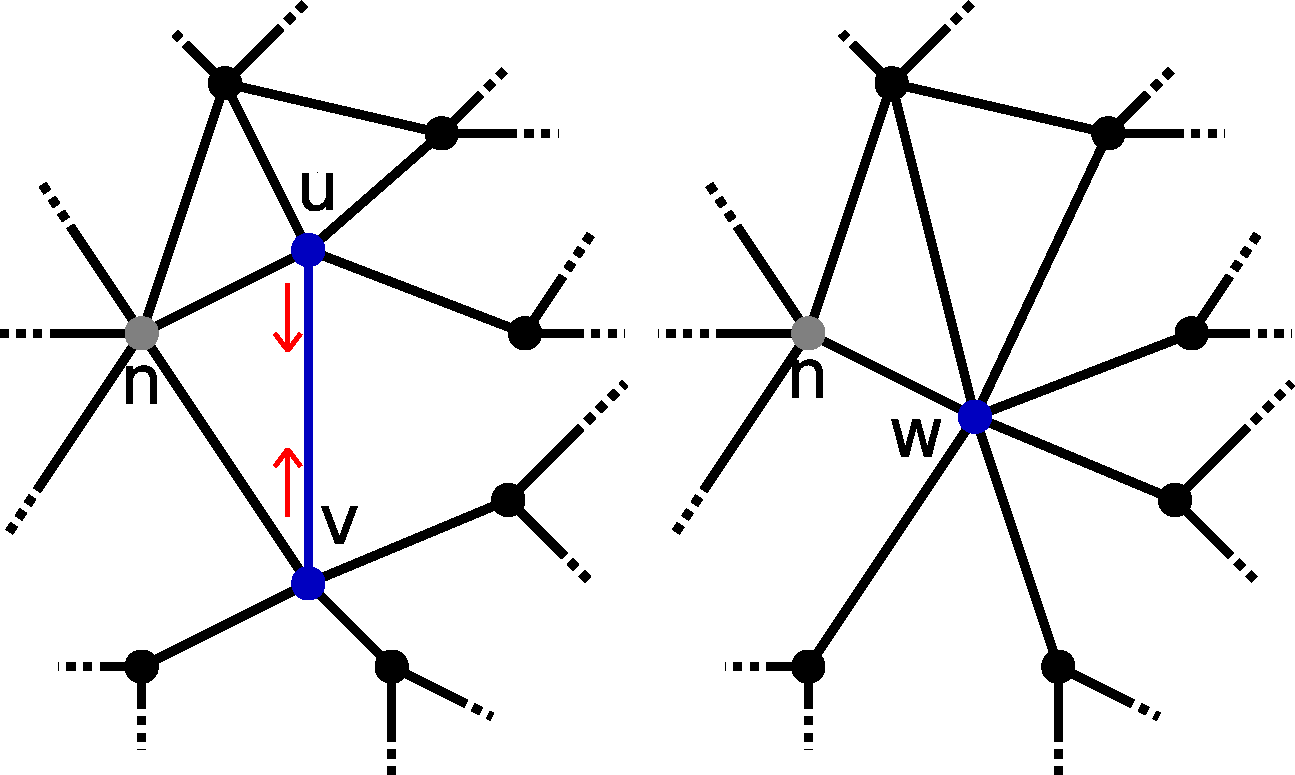
\includegraphics[width=0.35\textwidth]{fig/contraction.pdf}

    \addtocontents{lof}{%
        \vspace{1cm}
        \protect\centerline{%
            \protect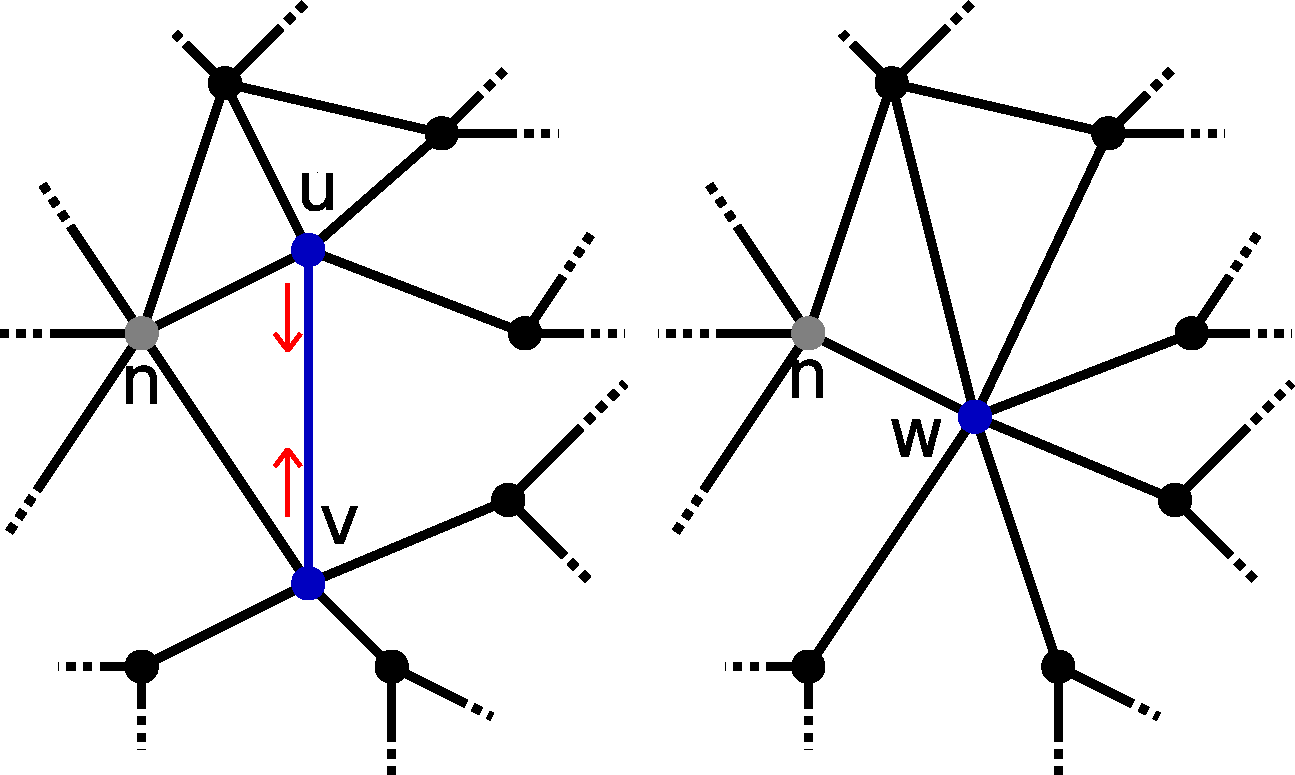
\includegraphics[width=\lofthumbsize,height=\lofthumbsize,keepaspectratio=true]{fig/contraction.pdf} 
        } 
    }%

    %\addtocontents{lof}{%
    %    $\vcenter to \lofthumbsize{\vss%
    %        \hbox to \lofthumbsize {
    %            \hss \protect 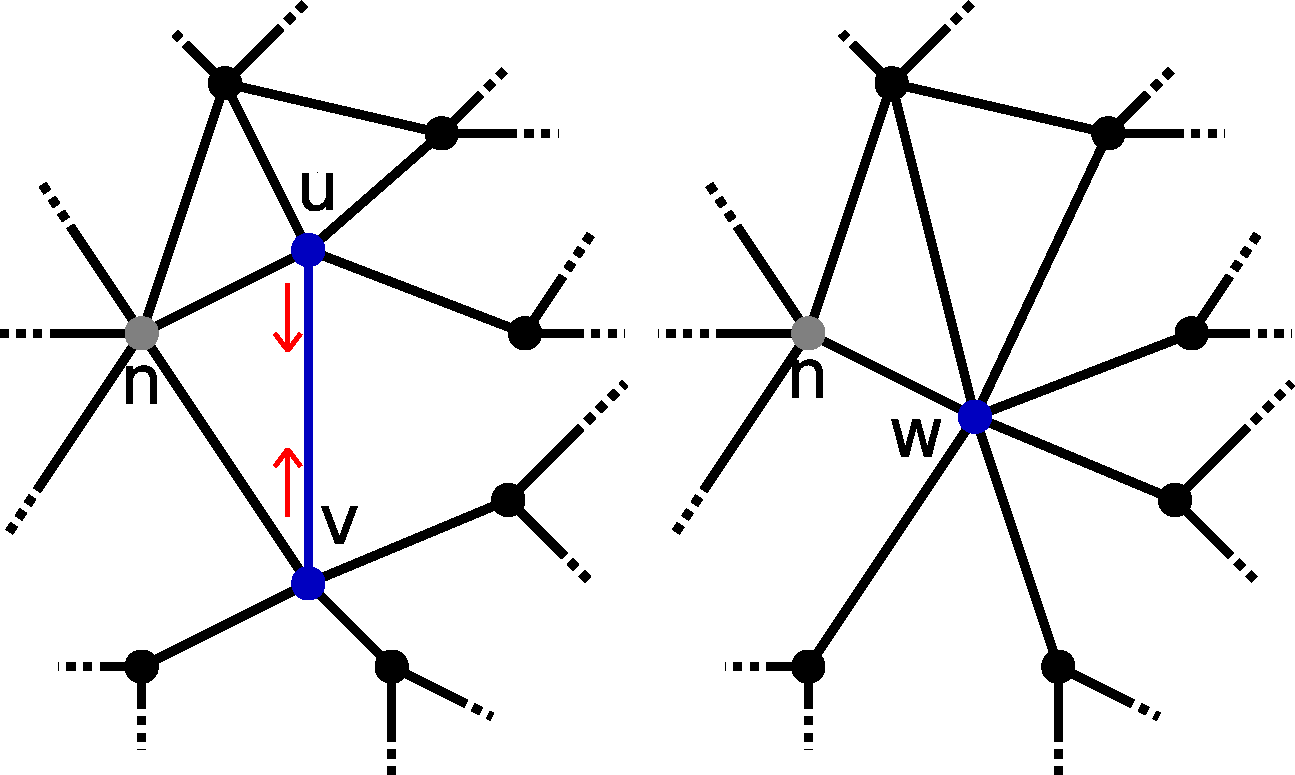
\includegraphics[width=.075\linewidth]{fig/contraction.pdf} \hss
    %        }
    %    \vss}$%
    %    \quad
    %    \ignorespaces
    %}%
    \caption[Schematic edge contraction]{ Schematic edge contraction: Node $u$ and $v$ is merged into node $w$.
        Note the gray node $n$ which is connected to $u$ and $v$.
        After the contraction, edges $\{ n,u\}$ and $\{ n,v\}$ are also merged into 
        a single edge $\{ n, w\}$ 
    }
    \label{fig:figlabel}
\end{figure}


   

\begin{center}
    \begin{tikzpicture}
        \umlclass[template=Graph]{MergeGraphAdpator}
        {
            \\// union find data structures                     \\
            - edgeUfd               : IterablePartiton          \\
            - nodeUfd               : IterablePartiton          \\ 
            - nodesAdjacency        : AdjacencySetVector        \\

            \\// callbacks                                      \\
            - mergeNodeCallBacks    : MergeNodeCallBackVector   \\
            - mergeEdgeCallBack     : MergeEdgeCallBackVector   \\
            - eraseEdgeCallBack     : EraseEdgeCallBackVector   \\
        }
        {
            \\// LEMON API for undirected graphs                \\
                $\ldots$                                        \\
            \\// register callbacks                             \\ 
            + registerMergeNodeCallBack(f : MergeNodeCallBack)  \\
            + registerMergeEdgeCallBack(f : MergeEdgeCallBack)  \\
            + registerEraseEdgeCallBack(f : EraseEdgeCallBack)  \\

            \\// modify graph                                   \\
            + contractEdge(edge : Edge)     : Node              \\

            \\// find representatives                           \\
            + reprNode(node : Node)         : Node              \\
            + reprEdge(edge : Edge)         : Edge              \\ 

            \\// get base graph                                 \\
            + graph()                       : Graph             \\
        } 
    \end{tikzpicture}
\end{center}

\begin{center}
    \begin{tikzpicture}
        \umlclass[template=MergeGraph]{ClusterOperatorInterface}
        {

        }
        {
            \\// contract next edge and get weight              \\
            + contractionEdge(edge : Edge)         : Edge       \\ 
            + contractionWeight(edge : Edge)       : Edge       \\
            \\// get base graph                                 \\
            + mergeGraph()                  : MergeGraph        \\
        } 
    \end{tikzpicture}
\end{center}

\begin{center}
    \begin{tikzpicture}
        \umlclass[template=ClusterOperator]{HierarchicalClustering}
        {

        }
        {
            + cluster()                     : void        \\
            + reprLabels(nodeMap : NodeMap) : void        \\      
        } 
    \end{tikzpicture}
\end{center}


   We propose and implemented the following design:
   \begin{compactitem}
       \item  A base graph is attached to a merge graph  and  a merge graph will
            always ``view'' to
       \item  Union find data structure for nodes
       \item  Union find data structure for edges
   \end{compactitem}



   \lstinline{vigra::MergeGraphAdaptor<DIM,DIRECTED_TAG>}


\subsection{Graph Algorithms} \label{sec:graph_graph_algorithms}

    \subsubsection{Multicut}

    \subsubsection{Hierarchical Clustering}

    \subsubsection{Mst Algorithms}

    \subsubsection{Watershed Algorithms}

    \subsubsection{Smoothing Algorithms}





\section{Python}




\begin{flushright}{\slshape    
(1) Beautiful is better than ugly. \\ \label{cit:line_a}
(2) Explicit is better than implicit. \\ \label{cit:line_b}
(3) Simple is better than complex. \\
(4) Complex is better than complicated. \\
(5) Flat is better than nested. \\
(6) Sparse is better than dense. \\
(7) Readability counts. \\
(8) Special cases aren't special enough to break the rules. \\
(9) Although practicality beats purity. \\
(10) Errors should never pass silently. \\
(11) Unless explicitly silenced. \\
(12) In the face of ambiguity, refuse the temptation to guess. \\
(13) There should be one-- and preferably only one --obvious way to do it. \\
(14) Although that way may not be obvious at first unless you're Dutch. \\
(15) Now is better than never. \\
(16) Although never is often better than *right* now. \\
(17) If the implementation is hard to explain, it's a bad idea. \\
(18) If the implementation is easy to explain, it may be a good idea. \\
(19) Namespaces are one honking great idea -- let's do more of those! } \\ \medskip
--- The Zen of Python
\end{flushright}
\captionof{figure}{ 
    The Zen of Python
}\label{fig:zen_of_python}






\subsection{Graph Maps}

On the python side, we want node-maps, edge-maps and arc-maps to be stored 
as numpy arrays for several reasons.
Numpy arrays are the standard for storing multidimensional data in python.
The fast C implementation and the highly vectorized API of numpy makes it very easy to write 
fast python code within a few lines.
Virtually any python user will be familiar with the numpy API and therefore it 
seems to be natural to store graph maps within numpy arrays.

In addition VIGRA provides an mechanism to pass numpy arrays to C++.
Therefore no new mechanism needs to be implemented to transfer graph
maps from python to C++.
This will not only simplify writing extension for the new VIGRA graph API,
but also it will reduce the glue code since we can use well tested existing
solutions.

New algorithms might be implemented in pure python with a mix of
existing numpy functions and new functions provided within VIGRA's graph API.
As a proof of concept we implemented ??? in pure python with VIGRA's
fresh graph API in \cref{???}.


\subsubsection{Intrinsic Graph Shape}

Each graph has an \emph{intrinsic node map shape} 
and an \emph{intrinsic edge map shape} and 
These intrinsic shape and dimensions are used to use 
numpy arrays with the best fitting dimension and shape.
For a 2D grid graph the node map should also be a 2D dimensional array.
because in this way an usual image can be used as an node map.
To access the  intrinsic shapes of node and edge maps 
we use a small trait class with default implementations
for unknown graphs.
The default implementation is given below:

\begin{minipage}{\textwidth}\vspace{-0.75cm}\begin{lstlisting}[language=c++]
template<class GRAPH>
class IntrinsicGraphShape{
private:
    typedef GRAPH Graph;
    typedef typename vigra::MultiArray<1,int>::difference_type DiffType1d;
    typedef typename Graph::index_type  index_type;
public:
    typedef typename Graph::Node Node ;
    typedef typename Graph::Edge Edge ;
    typedef typename  Graph::Arc  Arc ;

    typedef DiffType1d IntrinsicNodeMapShape;
    typedef DiffType1d IntrinsicEdgeMapShape;
    typedef DiffType1d  IntrinsicArcMapShape;

    static IntrinsicNodeMapShape intrinsicNodeMapShape(const Graph & g){
        return IntrinsicNodeMapShape(g.maxNodeId()+1);
    }
    static IntrinsicEdgeMapShape intrinsicEdgeMapShape(const Graph & g){
        return IntrinsicEdgeMapShape(g.maxEdgeId()+1);
    }
    static IntrinsicArcMapShape intrinsicArcMapShape(const Graph & g){
        return  IntrinsicArcMapShape(g.maxArcId()+1);
    }

    static const unsigned int IntrinsicNodeMapDimension=1;
    static const unsigned int IntrinsicEdgeMapDimension=1;
    static const unsigned int IntrinsicArceMapDimension=1;
};
\end{lstlisting}\end{minipage}\vspace{0.5cm}



\subsubsection{Numpy Arrays To LEMON Maps}


On the C++ side, numpy arrays are stored in MultiArrayViews.
Since the API of MultiArrayViews \cite{software_vigra_multiarray_api} does
not implemented the API  of LEMON graph maps (e.g. node-maps, edge-maps and arc-maps), 
a thin wrapper is used to convert the arrays to LEMON conform maps.
These wrappers can be accessed via \lstinline{PyNodeMapTraits<Graph,T>::Array} and 
\lstinline{PyNodeMapTraits<Graph,T>::Map}. 


In the following we will give a brief example how to pass numpy arrays to C++
and convert them to LEMON conform graph maps.

Assuming we need a function which does something with node features as normalization.
On the python side we want to have the following signature:

\lstinline{result=vigra.graphs.normNodeFeat(graph,nodeFeatures=nodeFeatures,out=None)}.

The function should work on single band node features and multi band node features
(an arbitrary number of channels, but the same for all nodes).
There should be a single C++ function which can be used to export
\lstinline{normNodeFeat} for any graph within VIGRA's graph API. 




\begin{minipage}{\textwidth}

To archive this we propose the following design:
On the C++ side we use a function  which
is has two templates , one for the graph, and one for the value type.
A prototypical implementation is given below.

\begin{minipage}{\textwidth}\vspace{-0.75cm}\begin{lstlisting}[language=c++]
template<class Graph,class T>
NumpyAnyArray normNodeFeat(
    const Graph & g,
    const typename PyNodeMapTraits<Graph,T >::Array & nodeFeaturesInArray,
    typename PyNodeMapTraits<Graph,T>::Array  outArray 
){
    // reshape out 
    // - last argument (outArray) will be reshaped if empty,
    // - and #channels is taken from second argument (nodeFeaturesIn) 
    reshapeNodeMapIfEmpty(g,nodeFeaturesIn,outArray);

    // numpy arrays => lemon maps 
    // featuresInMap and outMap fulfill
    // the concept of LEMON NODE MAPS
    typename PyNodeMapTraits<Graph,T >::Map featuresInMap(g,nodeFeaturesInArray);
    typename PyNodeMapTraits<Graph,T >::Map outMap(g,outArray);


    /* call code using LEMON API*/

    // return out as numpy array
    return outArray;
}
\end{lstlisting}\end{minipage}\vspace{0.5cm}

The template \lstinline{T} can be instantiated with scalars as \lstinline{float}, an explicit single band scalar as \lstinline{Singleband<float>}
or a multi band type as \lstinline{Multiband<float>}.

\lstinline{PyNodeMapTraits<Graph,T >::Array} will select the correct \lstinline{vigra::NumpyArray<DIM,VALUE_TYPE>} w.r.t.
the templates \lstinline{Graph} and \lstinline{T}.

The output array will be reshaped with the corrected number of channels by calling \lstinline{reshapeNodeMapIfEmpty}.
Equivalent functions exist for edge maps.

\lstinline{PyNodeMapTraits<Graph,T >::Map} is the corresponding LEMON conform  node map 
which is a cheap view to an numpy array. 
\end{minipage}


\begin{minipage}{\textwidth}
To make the function above available in python
we need to write wrapper code with \lstinline{boost::python}.
We will export the function for single band floats and multi band floats.

\begin{minipage}{\textwidth}\vspace{-0.75cm}\begin{lstlisting}[language=c++]
// single-band float32
boost::python::def(
    "normNodeFeat",
     &normNodeFeat<Graph,float>,
    (
        boost::python::arg("graph"),
        boost::python::arg("nodeFeatures"),
        boost::python::arg("out")=boost::python::object() // None
    )
);

// multi-band float32
boost::python::def(
    "normNodeFeat",
     &normNodeFeat<Graph,Multiband<float> >,
    (
        boost::python::arg("graph"),
        boost::python::arg("nodeFeatures"),
        boost::python::arg("out")=boost::python::object() // None
    )
);
\end{lstlisting}\end{minipage}\vspace{0.5cm}

\end{minipage}


On the python side we can call the function as desired.
The array which stores the result of this
function can be preallocated and passed explicitly.

\begin{minipage}{\textwidth}\vspace{-0.75cm}\begin{lstlisting}[language=Python]
// with automatically allocated outFeatures
outFeatures = vigra.graphs.normNodeFeat(graph,nodeFeatures)

// with explicitly given outFeatures
// - here we assume single band features
outFeatures2 = vigra.graphs.graphMap(graph,item='node',dtype=np.float32)
outFeatures2 = vigra.graphs.normNodeFeat(graph,nodeFeatures,out=outFeatures2)


// with multiband node features 
// - here we assume multi band features
//   with 3 channels per node
outFeatures2 = vigra.graphs.graphMap(graph,item='node',dtype=np.float32,channels=3)
outFeatures2 = vigra.graphs.normNodeFeat(graph,nodeFeatures,out=outFeatures2)
\end{lstlisting}\end{minipage}\vspace{0.5cm}




\subsection{Graph Hierarchy}
    
Explain the very nice workflow  

\part{Some Kind of Manual} % First part of the thesis

%!TEX root = <main.tex>
% Chapter 1

\chapter{Introduction} % Chapter title

\label{ch:introduction} % For referencing the chapter elsewhere, use \autoref{ch:introduction} 

%----------------------------------------------------------------------------------------


\section{Contribution}\label{sec:Contribution}


\begin{itemize}
    \item Fast Approximatively Multicut Solvers:

        An approximate solver for the multicut objective, 
        called Cut Clue and Cut (GCG) is proposed (see \ref{ch:multicut} ).
        Experiments show  that CGC is superior w.r.t. 
        runtime compared to state of the art solvers, and find solutions
        very close to global optimal solution (see \ref{ch:multicut_experiments}) 

    \item Generalized Fusion Moves:

        An generalization of fusion moves \cite{lempitsky_2010_pami}


    \item Implemented a Graph library and algorithms within vigra.


\end{itemize}




\section{Some Code stuff}
\begin{lstlisting}[language=python]
>>> from numpy import *
>>> from numpy.fft
\end{lstlisting}
\section{Some Tikz stuff}






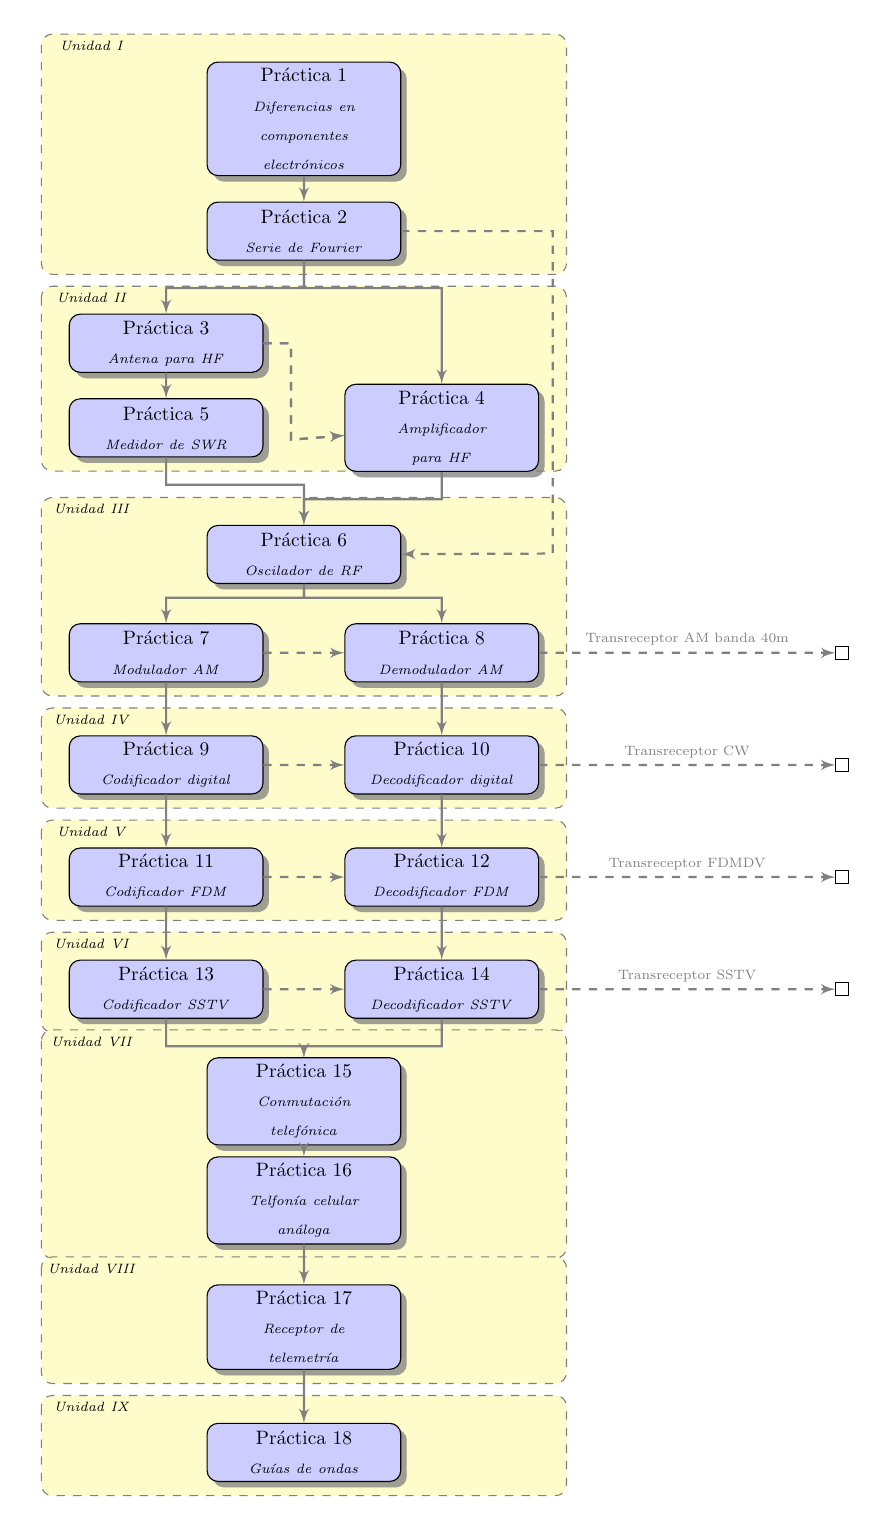
\begin{tikzpicture}[scale=0.7,transform shape]
 
  % Draw diagram elements
  \path \practica {1}{Diferencias en componentes electr\'onicos};
  \path (p1.south)+(0.0,-1.0) \practica{2}{Serie de Fourier};
  \path (p2.south)+(-2.5,-1.5) \practica{3}{Antena para HF};
  \path (p3.south)+(0.0,-1.0) \practica{5}{Medidor de SWR};
  \path (p3.south)+(5.0,-1.0) \practica{4}{Amplificador para HF};

  \path (p4.south)+(-2.5,-1.5) \practica{6}{Oscilador de RF};
  \path (p6.south)+(-2.5,-1.25) \practica{7}{Modulador AM};
  \path (p6.south)+(2.5,-1.25) \practica{8}{Demodulador AM};
  \path (p8.east)+(+5.5,0) node (ur1)[ur] {};

  \path (p7.south)+(0.0,-1.5) \practica{9}{Codificador digital};
  \path (p8.south)+(0.0,-1.5) \practica{10}{Decodificador digital};
  \path (p10.east)+(+5.5,0) node (ur2)[ur] {};
  \path (p9.south)+(0.0,-1.5) \practica{11}{Codificador FDM};
  \path (p10.south)+(0.0,-1.5) \practica{12}{Decodificador FDM};
  \path (p12.east)+(+5.5,0) node (ur3)[ur] {};
  \path (p11.south)+(0.0,-1.5) \practica{13}{Codificador SSTV};
  \path (p12.south)+(0.0,-1.5) \practica{14}{Decodificador SSTV};
  \path (p14.east)+(+5.5,0) node (ur4)[ur] {};
  \path (p14.south)+(-2.5,-1.5) \practica{15}{Conmutaci\'on telef\'onica};
  \path (p15.south)+(0.0,-1.0) \practica{16}{Telfon\'ia celular an\'aloga};
  \path (p16.south)+(0.0,-1.5) \practica{17}{Receptor de  telemetr\'ia}; 
  \path (p17.south)+(0.0,-1.5) \practica{18}{Gu\'ias de ondas};
     
  % Draw arrows between elements
  \path [line] (p1.south) -- node [above] {} (p2);

  \path [line] (p2.south) -- +(0.0,-0.5) -- +(-2.5,-0.5)
    -- node [above, midway] {} (p3);
  \path [line] (p3.south) -- node [above] {} (p5) ;
     
  \path [line] (p2.south) -- +(0.0,-0.5) -- +(+2.5,-0.5)
    -- node [above, midway] {} (p4);
  \path [linepart] (p3.east) -- +(+0.5,-0.0) -- +(+0.5,-1.75)
    -- node [left, midway] {} (p4);
  \path [linepart] (p3.east) -- +(+0.5,-0.0) -- +(+0.5,-1.75)
    -- node [left, midway] {} (p4);

  \path [line] (p4.south) -- +(0.0,-0.5) -- +(-2.5,-0.5)
    -- node [above, midway] {} (p6);
  \path [line] (p5.south) -- +(0.0,-0.5) -- +(+2.5,-0.5)
    -- node [above, midway] {} (p6);     
  \path [linepart] (p2.east) -- +(2.75,0.0) -- +(2.75,-5.85)
    -- node [right] {} (p6);
  \path [line] (p6.south) -- +(0.0,-0.25) -- +(-2.5,-0.25)
    -- node [above, midway] {} (p7);
  \path [line] (p6.south) -- +(0.0,-0.25) -- +(+2.5,-0.25)
    -- node [above, midway] {} (p8);
  \path [linepart] (p7.east) -- node [left] {} (p8);
  \transreceptor{p8}{AM banda 40m}{ur1}

  \path [line] (p7.south) -- node [above] {} (p9) ;
  \path [line] (p8.south) -- node [above] {} (p10) ;
  \path [linepart] (p9.east) -- node [left] {} (p10);
  \transreceptor{p10}{CW}{ur2}
  \path [line] (p9.south) -- node [above] {} (p11) ;
  \path [line] (p10.south) -- node [above] {} (p12) ;
  \path [linepart] (p11.east) -- node [left] {} (p12);
  \transreceptor{p12}{FDMDV}{ur3}

  \path [line] (p11.south) -- node [above] {} (p13) ;
  \path [line] (p12.south) -- node [above] {} (p14) ;
  \path [linepart] (p13.east) -- node [left] {} (p14);   
  \transreceptor{p14}{SSTV}{ur4}

  \path [line] (p14.south) -- +(0.0,-0.5) -- +(-2.5,-0.5)
    -- node [above, midway] {} (p15);
  \path [line] (p13.south) -- +(0.0,-0.5) -- +(+2.5,-0.5)
    -- node [above, midway] {} (p15);
  \path [line] (p15.south) -- node [above] {} (p16) ;     
  \path [line] (p16.south) -- node [above] {} (p17) ;
  \path [line] (p17.south) -- node [above] {} (p18) ;
   
  \background{p3}{p1}{p4}{p2}{I}
  \background{p3}{p3}{p4}{p5}{II}
  \background{p3}{p6}{p4}{p7}{III}
  \background{p3}{p9}{p4}{p10}{IV}
  \background{p3}{p11}{p4}{p12}{V}
  \background{p3}{p13}{p4}{p14}{VI}
  \background{p3}{p15}{p4}{p16}{VII}
  \background{p3}{p17}{p4}{p17}{VIII}
  \background{p3}{p18}{p4}{p18}{IX}
\end{tikzpicture}




















\begin{center}
\begin{tabular}{l|ll}
bla & set & vector\\ \hline

denk-450           
& 1.0 & 2.0\\
denk-450 ward         
& 1.0 & 5.0\\

bsd-500           
& 1.0 & 2.0\\
bsd-500 ward         
& 1.0 & 5.0

\end{tabular}
\end{center}



\begin{tikzpicture}[scale=  1,every node/.style={minimum size=1cm},on grid]
        
    %slanting: production of a set of n 'laminae' to be piled up. N=number of grids.
    

    %%%%%%%%%%%%%%%%%%%%%%%%%%%%%%%%%%%%%%%%%%%%%%%%%%%%%%%%%%%%%%%
    % 0 bottom layer
    %%%%%%%%%%%%%%%%%%%%%%%%%%%%%%%%%%%%%%%%%%%%%%%%%%%%%%%%%%%%%%%%
        
    \begin{scope}[
        yshift=0,every node/.append style={
            yslant=0.5,xslant=-1},yslant=0.5,xslant=-1
                     ]
        
        \draw[-latex,thick] (-0.17,2.5) node[right]{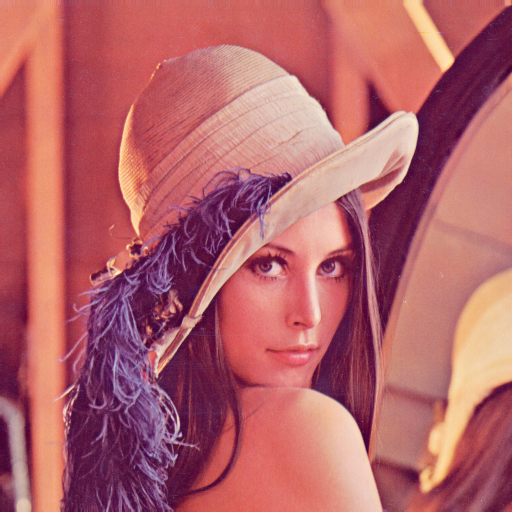
\includegraphics[width=5cm]{fig/lena.png}};
        \fill[white,fill opacity=.0] (0,0) rectangle (5,5);
        \draw[black,very thick] (0,0) rectangle (5,5);
        \draw[step=1.8mm, black] (0,0) grid (5,5);
    \end{scope}

    %%%%%%%%%%%%%%%%%%%%%%%%%%%%%%%%%%%%%%%%%%%%%%%%%%%%%%%%%%%%%%%
    % 1 layer
    %%%%%%%%%%%%%%%%%%%%%%%%%%%%%%%%%%%%%%%%%%%%%%%%%%%%%%%%%%%%%%%%
    
   \begin{scope}[
        yshift=100,every node/.append style={
            yslant=0.5,xslant=-1},yslant=0.5,xslant=-1
                     ]
        
        \draw[-latex,thick] (-0.17,2.5) node[right]{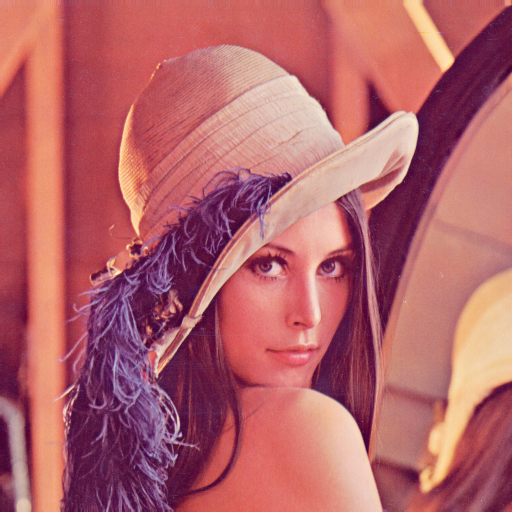
\includegraphics[width=5cm]{fig/lena.png}};
        \fill[white,fill opacity=.0] (0,0) rectangle (5,5);
        \draw[black,very thick] (0,0) rectangle (5,5);
        \draw[step=1.8mm, black] (0,0) grid (5,5);
    \end{scope}
        
     %%%%%%%%%%%%%%%%%%%%%%%%%%%%%%%%%%%%%%%%%%%%%%%%%%%%%%%%%%%%%%%
    % 2 layer
    %%%%%%%%%%%%%%%%%%%%%%%%%%%%%%%%%%%%%%%%%%%%%%%%%%%%%%%%%%%%%%%%
    
   \begin{scope}[
        yshift=200,every node/.append style={
            yslant=0.5,xslant=-1},yslant=0.5,xslant=-1
                     ]
        
        \draw[-latex,thick] (-0.17,2.5) node[right]{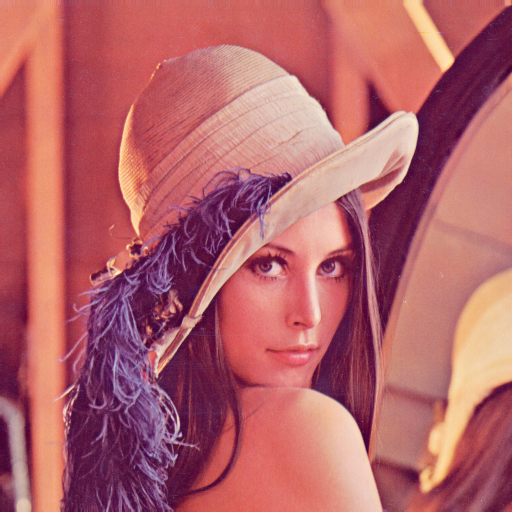
\includegraphics[width=5cm]{fig/lena.png}};
        \fill[white,fill opacity=.0] (0,0) rectangle (5,5);
        \draw[black,very thick] (0,0) rectangle (5,5);
        \draw[step=1.8mm, black] (0,0) grid (5,5);
    \end{scope}
        


    %%%%%%%%%%%%%%%%%%%%%%%%%%%%%%%%%%%%%%%%%%%%%%%%%%%%%%%%%%%%%%%
    % 0 bottom layer
    %%%%%%%%%%%%%%%%%%%%%%%%%%%%%%%%%%%%%%%%%%%%%%%%%%%%%%%%%%%%%%%%
    \draw[-latex,thick] (6.2,2) node[right]{$\mathsf{Grid Graph}$}
         to[out=180,in=90] (4,2);
         
         
         
    %%%%%%%%%%%%%%%%%%%%%%%%%%%%%%%%%%%%%%%%%%%%%%%%%%%%%%%%%%%%%%%
    % 1 layer
    %%%%%%%%%%%%%%%%%%%%%%%%%%%%%%%%%%%%%%%%%%%%%%%%%%%%%%%%%%%%%%%%
    
    \draw[-latex,thick] (6.2,5.5) node[right]{$\mathsf{Region adjacency graph 1}$}
         to[out=180,in=90] (4,5.5);

\end{tikzpicture}






































% We need layers to draw the block diagram
\pgfdeclarelayer{background}
\pgfdeclarelayer{foreground}
\pgfsetlayers{background,main,foreground}

% Define a few styles and constants
\tikzstyle{sensor}=[draw, fill=blue!20, text width=5em, 
    text centered, minimum height=2.5em]
\tikzstyle{ann} = [above, text width=5em]
\tikzstyle{naveqs} = [sensor, text width=6em, fill=red!20, 
    minimum height=12em, rounded corners]
\def\blockdist{2.3}
\def\edgedist{2.5}

\begin{tikzpicture}
    \node (naveq) [naveqs] {Navigation equations};
    % Note the use of \path instead of \node at ... below. 
    \path (naveq.140)+(-\blockdist,0) node (gyros) [sensor] {Gyros};
    \path (naveq.-150)+(-\blockdist,0) node (accel) [sensor] {Accelero-meters};
    
    % Unfortunately we cant use the convenient \path (fromnode) -- (tonode) 
    % syntax here. This is because TikZ draws the path from the node centers
    % and clip the path at the node boundaries. We want horizontal lines, but
    % the sensor and naveq blocks aren't aligned horizontally. Instead we use
    % the line intersection syntax |- to calculate the correct coordinate
    \path [draw, ->] (gyros) -- node [above] {$\vc{\omega}_{ib}^b$} 
        (naveq.west |- gyros) ;
    % We could simply have written (gyros) .. (naveq.140). However, it's
    % best to avoid hard coding coordinates
    \path [draw, ->] (accel) -- node [above] {$\vc{f}^b$} 
        (naveq.west |- accel);
    \node (IMU) [below of=accel] {IMU};
    \path (naveq.south west)+(-0.6,-0.4) node (INS) {INS};
    \draw [->] (naveq.50) -- node [ann] {Velocity } + (\edgedist,0) 
        node[right] {$\vc{v}^l$};
    \draw [->] (naveq.20) -- node [ann] {Attitude} + (\edgedist,0) 
        node[right] { $\mx{R}_l^b$};
    \draw [->] (naveq.-25) -- node [ann] {Horisontal position} + (\edgedist,0)
        node [right] {$\mx{R}_e^l$};
    \draw [->] (naveq.-50) -- node [ann] {Depth} + (\edgedist,0) 
        node[right] {$z$};
    
    % Now it's time to draw the colored IMU and INS rectangles.
    % To draw them behind the blocks we use pgf layers. This way we  
    % can use the above block coordinates to place the backgrounds   
    \begin{pgfonlayer}{background}
        % Compute a few helper coordinates
        \path (gyros.west |- naveq.north)+(-0.5,0.3) node (a) {};
        \path (INS.south -| naveq.east)+(+0.3,-0.2) node (b) {};
        \path[fill=yellow!20,rounded corners, draw=black!50, dashed]
            (a) rectangle (b);
        \path (gyros.north west)+(-0.2,0.2) node (a) {};
        \path (IMU.south -| gyros.east)+(+0.2,-0.2) node (b) {};
        \path[fill=blue!10,rounded corners, draw=black!50, dashed]
            (a) rectangle (b);
    \end{pgfonlayer}
\end{tikzpicture}


















\centering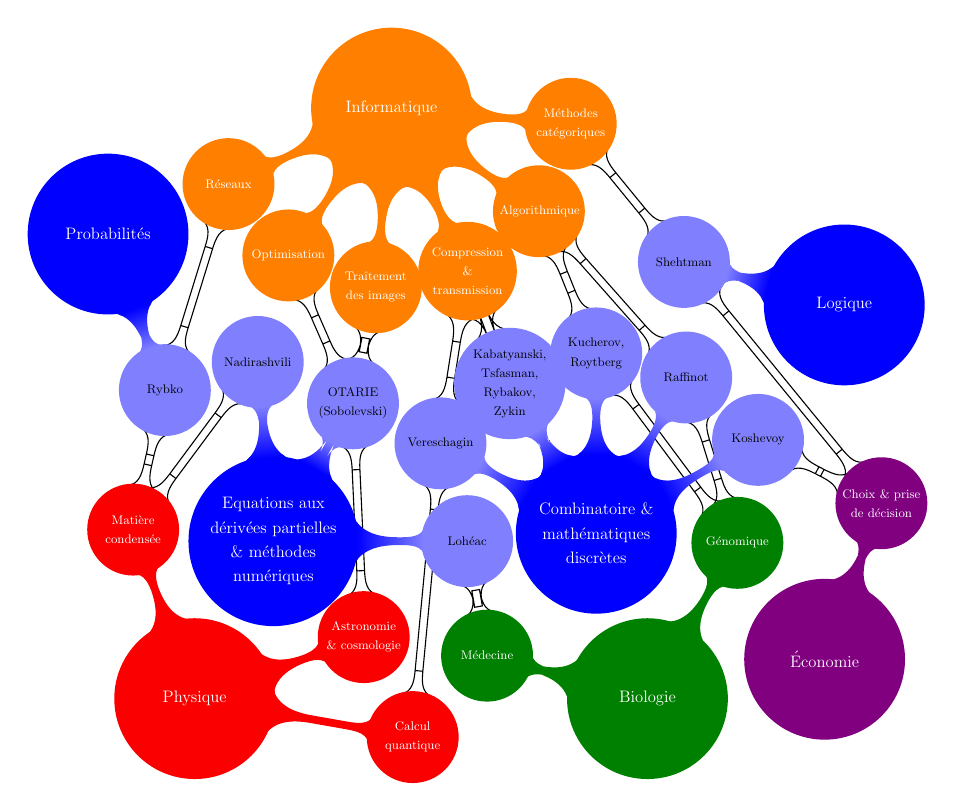
\begin{tikzpicture}[mindmap,scale=0.5, transform shape,
  level 1 concept/.append style={level distance=130,sibling angle=30},
  extra concept/.append style={color=blue!50,text=black}]
  % Applied area: computer science and its subfields

  \begin{scope}[mindmap, concept color=orange, text=white]
    \node [concept] {Informatique}[clockwise from=-5] 
      child {node [concept] (log) {M{\'e}thodes cat{\'e}goriques}}
      child {node [concept] (alg) {Algorithmique}}
      child {node [concept] (cod) {Compression \& transmission}}
      child {node [concept] (img) {Tra{\^i}tement des images}}
      child {node [concept] (opt) {Optimisation}}
      child {node [concept] (res) {R{\'e}seaux}};
  \end{scope}

  % Applied area: theoretical physics and its subfields

  \begin{scope}[mindmap, concept color=red,text=white]
    \node [concept] at (-5,-15) {Physique}
      child [grow=-10, level distance=160]
        {node [concept] (qin) {Calcul quantique}}
      child [grow=20] 
        {node [concept] (csm) {Astronomie \& cosmologie}}
      child [grow=110] 
        {node [concept] (mat) {Mati{\`e}re condens{\'e}e}};
  \end{scope}

  % Applied area: biology and its subfields

  \begin{scope}[mindmap, concept color=green!50!black,text=white]
    \node [concept] at (6.5,-15) {Biologie} 
      child [grow=165, level distance=120] 
        {node [concept] (med) {M{\'e}decine}}
      child [grow=60] 
        {node [concept] (gen) {G{\'e}nomique}};
  \end{scope}

  % Applied area: economics (one subfield)

  \begin{scope}[mindmap, concept color=violet, text=white]
    \node [concept] at (11,-14) {{\'E}conomie}
      child [grow=70, level distance=120] 
        {node [concept] (dec) {Choix \& prise de d{\'e}cision}};
  \end{scope}

  % Researchers listed by their main specialization in mathematics

  \begin{scope}[mindmap, concept color=blue]

    % Combinatorics and discrete mathematics 
    \node [concept, text=white] at (5.2,-10.8) 
      {Combinatoire \& math{\'e}matiques discr{\`e}tes} 
      [clockwise from=150]
      child [concept color=blue!50] {node [concept] (ver) {Vereschagin}}
      child [concept color=blue!50, level distance=125] 
        {node [concept] (kab) {Kabatyanski, Tsfasman, Rybakov, Zykin}}
      child [concept color=blue!50] 
        {node [concept] (kch) {Kucherov, Roytberg}}
      child [concept color=blue!50] {node [concept] (raf) {Raffinot}}
      child [concept color=blue!50, level distance=135]
        {node [concept] (ksh) {Koshevoy}};

    % Partial differential equations
    \node [concept, text=white] at (-3,-11) 
      {Equations aux d{\'e}riv{\'e}es partielles 
        \& m{\'e}thodes num{\'e}riques}
      child [concept color=blue!50, grow=0, level distance=140] 
        {node [concept] (lhc) {Loh{\'e}ac}}
      child [concept color=blue!50, grow=60, level distance=115] 
        {node [concept] (otr) {OTARIE (Sobolevski)}}
      child [concept color=blue!50, grow=95] {node [concept] (ndr) 
        {Nadirashvili}};

    % Probability
    \node [concept, text=white] at (-7.2,-3.2) {Probabilit{\'e}s}
      child [concept color=blue!50, grow=-70, level distance=120] 
        {node [concept] (rbk) {Rybko}};

    % Logic
    \node [concept, text=white] at (11.5,-5) {Logique}
      child [concept color=blue!50, grow=165, level distance=120] 
        {node [concept] (sht) {Shehtman}};
  \end{scope}

  % Connections of researchers to applied subfields

  \begin{pgfonlayer}{background}
    \draw [circle connection bar]
      (kab) edge (cod)
      (kch) edge (alg) edge (gen)
      (lhc) edge (med)
      (ksh) edge (dec)
      (ndr) edge (mat)
      (otr) edge (opt) edge (csm) edge (img)
      (raf) edge (alg) edge (gen)
      (rbk) edge (res) edge (mat)
      (sht) edge (log) edge (dec)
      (ver) edge (qin) edge (cod);
  \end{pgfonlayer}

\end{tikzpicture}


\newpage





% Below we mix an ordinary equation with TikZ nodes. Note that we have to
% adjust the baseline of the nodes to get proper alignment with the rest of
% the equation.
\begin{equation}
\omega_{e} = 
        \tikz[baseline]{\node[fill=blue!20,anchor=base] (te)        
            {$ f_{\epsilon}(X_{e}) $};
        } +
        \tikz[baseline]{\node[fill=red!20,anchor=base] (tuv)
            {$  d_{\nu}(X_u,X_v) $};
        } +   
        \tikz[baseline]{ \node[fill=green!20,anchor=base] (tr)
            {$r(|u|,|v|,|e|)$};  
        }
\end{equation}

\begin{itemize}
    \item Edge indicator:          \tikz\node [fill=blue!20,draw,circle] (ne) {};
        \begin{itemize}
         \item Gradient magnitude
         \item Eigenvalues of hessian
        \end{itemize}
    \item Node feature difference: \tikz\node [fill=red!20,draw,circle] (nuv) {};
       \begin{itemize}
         \item L1,L2
         \item Histogram differences ($\chi^2$,Earth movers distance)
       \end{itemize}
    \item Geometric regularizer:   \tikz\node [fill=green!20,draw,circle] (nr) {};
       \begin{itemize}
         \item Wards criterion \cite{ward_clustering}
         \item Log Ward criterion
         \item None 
      \end{itemize}
\end{itemize}

% Now it's time to draw some edges between the global nodes. Note that we
% have to apply the 'overlay' style.
%\begin{tikzpicture}[overlay]
%        \path[->] (ne) edge [bend right] (te);
%        \path[->] (nuv) edge [bend right] (tuv);
%        \path[->] (nr) edge [out=0, in=-90] (tr);
%\end{tikzpicture}



% -------------------------------------------------
% Set up a new layer for the debugging marks, and make sure it is on
% top
\pgfdeclarelayer{marx}
\pgfsetlayers{main,marx}
% A macro for marking coordinates (specific to the coordinate naming
% scheme used here). Swap the following 2 definitions to deactivate
% marks.
\providecommand{\cmark}[2][]{%
  \begin{pgfonlayer}{marx}
    \node [nmark] at (c#2#1) {#2};
  \end{pgfonlayer}{marx}
  } 
\providecommand{\cmark}[2][]{\relax} 


 % Chapter 1

\cleardoublepage % Empty page before the start of the next part

%------------------------------------------------

\ctparttext{You can put some informational part preamble text here. Illo principalmente su nos. Non message \emph{occidental} angloromanic da. Debitas effortio simplificate sia se, auxiliar summarios da que, se avantiate publicationes via. Pan in terra summarios, capital interlingua se que. Al via multo esser specimen, campo responder que da. Le usate medical addresses pro, europa origine sanctificate nos se.} % Text on the Part 2 page describing the content in Part 2

\part{The Showcase} % Second part of the thesis

% Chapter 1
\flushleft
\chapter{Multicut}\label{ch:multicut} 

\section{Motivation}\label{sec:mc_motivation}


\section{Problem Formulation}\label{sec:mc_problem_formulation}


Given a graph $G=(V,E)$ and an edge weight $w_e  \forall e \in E $ .
A negative edge weight indicates that $u_e$ and $v_e$ should be
disconnected while a positive edge weight indicated that $u_e$ and $v_e$ should be in the same cluster. Therefore an edge with a negative edge should be cut, while positive edges should stay uncut.

Let $X_E \in \{0,1\}^{|E|}$ be an edge labeling where $x_e=1$ means an edge is
cut and $x_e=0$ mean the edge is uncut. 

\todo{how $X_E$ induces X}





\section{Cutting Planes Multicut}\label{sec:cp_multicut}

Describe Joergs Multicut here





While the multicut objective is very simple and elegant, it is very
hard to optimize such an objective to global optimality.
In fact, solving the multicut to optimality is $\mathcal{NP}$-hard \cite{???} 
\todo{who to cite on multicut $\mathcal{NP}$ hardness}.
It has been showed that even such $\mathcal{NP}$-hard problems can
be solved to optimality \cite{andres_2011_iccv,kappes_2011_emmcvpr}, but still,
global optimal solvers are far way from a \todo{a speed , or just speed} speed which would be necessary for
real time segmentation, at least for  graphs with more than a few thousands nodes. 
Approximative solvers exists, but they are a) still to slow, and or b) far away from the global optimal solution (see figure \ref{fig:???} and table \ref{tab:???}).

\section{Cut Glue and Cut}



\subsection{Algorithm}

    \begin{algorithm}
        \ifx\DontPrintSemicolon\undefined
        \else
        \DontPrintSemicolon
        \fi
        \KwData{weighted graph $G=(V,E,\w)$,
                segmentation into regions given as queue $Q$}
        \KwResult{segmentation into smaller regions $Q'$}
        %
        $Q' \leftarrow \emptyset$\;
        %
        \While{$Q\neq\emptyset$}{
            $R \leftarrow \text{queue\_pop}(Q)$\;
            $\y_{E_R}$ $\leftarrow$ solve max-cut \eqref{eq:max_cut} for $G_R$\;
            \If{$\CUT_{G_R}(\y_{E_R}) < 0$}{
                $Q \leftarrow Q \cup \text{connected\_components}(\y_{E_R})$\;
            }
            \Else{
                $Q' \leftarrow Q' \cup R$
            }
        }
        \caption{Cut phase\label{alg:cut_phase}}

    \end{algorithm}


    \begin{algorithm}[t]
        \ifx\DontPrintSemicolon\undefined
        \else
        \DontPrintSemicolon
        \fi
        \KwData{weighted graph $G\!=\!(V,E,\w)$, segmentation $Q$}
        \KwResult{improved segmentation $Q$ wrt. \eqref{eq:multicut_primal}}
        %
        mark all edges $e\in E$ as dirty\;
        $\bar{\y} \leftarrow \text{edge\_labeling}(Q)$\;
        \While{true}{\label{alg:line:forever}%
            $c \leftarrow 0$\;
            $E' \leftarrow \{ e\in E\cap (R_1 \times R_2) | R_1,R_2\in Q\text{ adjacent}\}$\footnotemark\label{alg:line:e_dash}\;
            \For{$e=(i,j)\in E'$}{
                \If{$\bar{\y}_e=0$ or $e$ is clean}{
                    continue\; 
                }
                find regions $R_1, R_2\!\in\!Q$, s.t. $i\in R_1$, $j\in R_2$\;
                $S \leftarrow R_1 \cup R_2\quad\text{//glue}$\;
                $\y_{E_S}$ $\leftarrow$ solve \eqref{eq:max_cut} for $G_S\quad\text{//cut}$\;
                {\color{blue}mark edges $E \cap S\times S$ clean$\quad(\star)$}\;
                \If{$\CUT_{G_S}(\y_{E_S}) < \CUT_{G_S}(\bar{\y}_{E_S})$}{
                    $c \leftarrow c+1$\;
                    {\color{blue}mark edges $E \cap S \times (V\setminus S)$ dirty$\quad(\star)$}\;
                    $\text{CC} \leftarrow \text{connected\_components}(\y_{E_S})$\;
                    {\color{blue}
                    \If{$|\CC| > 2$}{
                        mark edges $E \cap (S\times S)$ dirty$\quad(\star)$\;
                    }}
                    $Q \leftarrow Q\setminus \{R_1, R_2\} \cup \text{CC}$\;
                    $\bar{\y} \leftarrow \text{edge\_labeling}(Q)$\;
                }
            }
            \If{$c = 0$}{
                break\label{alg:line:break}\;
            }
        }
        %
        \caption{Glue \& Cut phase\label{alg:glue_cut_phase}}
    \end{algorithm}


    \begin{algorithm}
        \ifx\DontPrintSemicolon\undefined
        \else
        \DontPrintSemicolon
        \fi
        \KwData{weighted graph $G=(V,E,\w)$,
                segmentation into regions given as queue $Q$}
        \KwResult{segmentation into smaller regions $Q'$}
        $\quad\text{//TODO}$
        \caption{Pseudo min-marginals \label{alg:cgc_min_marginals}}

    \end{algorithm}


    Here comes the pseudocode for cut glue and cut min marginals

\subsection{Experiments}







 
% Chapter 1

\chapter{Hierarchical Clustering}\label{ch:hierarchical_clustering} 

\subsection{Motivation}\label{sec:hc_motivation}
why hclsutering and not multicut or naive thresholding


\subsection{Motivation}\label{sec:hc_motivation}
why hclsutering and not multicut or naive thresholding.


Agglomeration:


The main reason for the success of hierarchical clustering 
is the fact that agglomeration can be applied.

\begin{figure}[h]
 \missingfigure{principle of agglomeration}
\end{figure}





\subsection{Ultrametric Contour Map}{sec:ucm}

\begin{aenumerate} 
\item show basic algorithms 
\item explain concept of cluster operator
\item why we do not want this
\item show ucm with th
\end{aenumerate}

\missingfigure{ show ucm with wide and non wide boundary indicators}

\subsection{Implementation}

 
%\include{Chapters/Chapter02} % Chapter 2
%\include{Chapters/Chapter03} % Chapter 3
%\include{Chapters/Chapter04} % Chapter 4 - empty template

%----------------------------------------------------------------------------------------
%	THESIS CONTENT - APPENDICES
%----------------------------------------------------------------------------------------

\appendix

\part{Appendix} % New part of the thesis for the appendix

\include{Chapters/Chapter0A} % Appendix A
%\include{Chapters/Chapter0B} % Appendix B - empty template

%----------------------------------------------------------------------------------------
%	POST-CONTENT THESIS PAGES
%----------------------------------------------------------------------------------------

\cleardoublepage% Bibliography

\label{app:bibliography} % Reference the bibliography elsewhere with \autoref{app:bibliography}

\manualmark
\markboth{\spacedlowsmallcaps{\bibname}}{\spacedlowsmallcaps{\bibname}} 
\refstepcounter{dummy}

\addtocontents{toc}{\protect\vspace{\beforebibskip}} % Place the bibliography slightly below the rest of the document content in the table of contents
\addcontentsline{toc}{chapter}{\tocEntry{\bibname}}

\bibliographystyle{plainnat}

\bibliography{Bibliography} % Bibliography

%\cleardoublepage% Colophon (a brief description of publication or production notes relevant to the edition)

\pagestyle{empty}

\hfill

\vfill

\pdfbookmark[0]{Colophon}{colophon}

\section*{Colophon}

This document was typeset using the typographical look-and-feel \texttt{classicthesis} developed by Andr\'e Miede. The style was inspired by Robert Bringhurst's seminal book on typography ``\emph{The Elements of Typographic Style}''. \texttt{classicthesis} is available for both \LaTeX\ and \mLyX: 

\begin{center}
\url{http://code.google.com/p/classicthesis/}
\end{center}

\noindent Happy users of \texttt{classicthesis} usually send a real postcard to the author, a collection of postcards received so far is featured here: 

\begin{center}
\url{http://postcards.miede.de/}
\end{center}
 
\bigskip

\noindent\finalVersionString % Colophon

%\cleardoublepage% Declaration

\refstepcounter{dummy}
\pdfbookmark[0]{Declaration}{declaration} % Bookmark name visible in a PDF viewer

\chapter*{Declaration} % Declaration section text

\thispagestyle{empty}

Put your declaration here.
\bigskip
 
\noindent\textit{\myLocation, \myTime}

\smallskip

\begin{flushright}
\begin{tabular}{m{5cm}}
\\ \hline
\centering\myName, \today \\
\end{tabular}
\end{flushright}
 % Declaration

%----------------------------------------------------------------------------------------

\end{document}
